\documentclass{ieeeaccess}

\usepackage{cite}
\usepackage{amsmath,amssymb,amsfonts}
\usepackage{algorithmic}
\usepackage{graphicx}
\usepackage{textcomp}
\usepackage{amsmath,amssymb,amsfonts}
\usepackage[normalem]{ulem}
\usepackage{environ}
% Revision markup: deleted = red + strikethrough, revised = blue
\newcommand{\revised}[1]{{\color[rgb]{0,0,1}#1}}
\newcommand{\deleted}[1]{{\color[rgb]{1,0,0}#1}}

% Block deletions: red text (strikethrough is not compatible with floats/citations)
\NewEnviron{revisedblock}{%
  \begingroup
  \color[rgb]{0,0,1}%
  \BODY
  \endgroup
}
\NewEnviron{deletedblock}{%
  \begingroup
  \color[rgb]{1,0,0}%
  \BODY
  \endgroup
}

% \newcommand{\deletedsubsection}[1]{\subsection*{{\color[rgb]{1,0,0}#1}}}
% \newcommand{\deletedsubsubsection}[1]{\subsubsection*{{\color[rgb]{1,0,0}#1}}}

\usepackage{algorithm}
\usepackage{array}
\usepackage[caption=false,font=footnotesize]{subfig}
\usepackage{stfloats}
\usepackage[hyphens]{url}
\usepackage{verbatim}
\usepackage{spverbatim}
\usepackage{bm}
\usepackage[font=footnotesize,labelfont=sf,textfont=sf]{subcaption}
\usepackage{booktabs}


% 追加で必要なもの
\usepackage{wrapfig}       % 図の回り込み
\usepackage{multirow}      % 表の複数行セル
\usepackage[normalem]{ulem} % 下線等を使う場合（emphと併用注意）

\usepackage{color}

\definecolor{accessblue}{cmyk}{1,0.5,0,0}
\makeatletter
\long\def\@makecaption#1#2{
\ifx\@captype\ftype@table%
\begin{flushleft}
\vspace*{5pt}
\parbox{\columnwidth}{\vss{\color{accessblue}\tablecapheadfont #1. \ }\raggedright\tablecapfont#2\vss}%
\end{flushleft}
\else%
\begin{flushleft}
\vspace*{5pt}
\parbox{\columnwidth}{\vss{\color{accessblue}\figcapheadfont #1. \ }\raggedright\figcapfont#2\vss}%
\end{flushleft}
\fi}
\makeatother

\makeatletter
\AtBeginDocument{\DeclareMathVersion{bold}
\SetSymbolFont{operators}{bold}{T1}{times}{b}{n}
\SetSymbolFont{NewLetters}{bold}{T1}{times}{b}{it}
\SetMathAlphabet{\mathrm}{bold}{T1}{times}{b}{n}
\SetMathAlphabet{\mathit}{bold}{T1}{times}{b}{it}
\SetMathAlphabet{\mathbf}{bold}{T1}{times}{b}{n}
\SetMathAlphabet{\mathtt}{bold}{OT1}{pcr}{b}{n}
\SetSymbolFont{symbols}{bold}{OMS}{cmsy}{b}{n}
\renewcommand\boldmath{\@nomath\boldmath\mathversion{bold}}}
\makeatother

\def\BibTeX{{\rm B\kern-.05em{\sc i\kern-.025em b}\kern-.08em
    T\kern-.1667em\lower.7ex\hbox{E}\kern-.125emX}}

%Your document starts from here ___________________________________________________
\begin{document}
\history{Date of publication xxxx 00, 0000, date of current version xxxx 00, 0000.}
\doi{10.1109/ACCESS.2024.0429000}

\title{Classification of postures of people with hand movement working in office environment by LiDAR sensor network}
\author{
  \uppercase{Wataru Sano}\authorrefmark{1},
  \uppercase{Jumpei Watanabe}\authorrefmark{2},
  \uppercase{Haruma Shiraishi}\authorrefmark{3},
  \uppercase{Ryusei Sugano}\authorrefmark{4}, \IEEEmembership{Graduate Student Member, IEEE},
  \uppercase{Ryoichi Shinkuma}\authorrefmark{5, 6}, \IEEEmembership{Senior Member, IEEE},
  \uppercase{Gabriele Trovato}\authorrefmark{7}, \IEEEmembership{Associate Member, IEEE}
}


\address[1]{Shibaura Institute of Technology, Tokyo, Japan}
\address[2]{Hyper Digital Twins Co., Ltd., Tokyo, Japan}

\tfootnote{This work was supported in part by JSPS KAKENHI, Japan, under Grant Nos. 23H00464 and 25H01124.}

\markboth
{J.Watanabe \headeretal: Classification of postures of people with hand movement working in office environment by LiDAR sensor network}
{J.Watanabe \headeretal: Classification of postures of people with hand movement working in office environment by LiDAR sensor network}

\corresp{Corresponding author: Wataru Sano (e-mail: al20104@shibaura-it.ac.jp).}


\begin{abstract}
  %1st paragraph
%1.
\deleted{This paper proposes an edge computing system for classifying postures with hand movement of office workers, which was left as a remaining issue in prior work, using a light detection-and-ranging (LiDAR) sensor network.}
\revised{An edge computing system is proposed for classifying postures with hand movement of office workers using a light detection-and-ranging (LiDAR) sensor network.}
%1-1
\deleted{The proposed system utilizes the LiDAR sensor network to acquire human poses with hand movement and performs preprocessing steps including trimming, calibration, feature estimation, clustering, and normalization.}
\deleted{%1-2.
It then classifies the postures by using deep learning.}
\revised{The system acquires human poses with hand movement through the LiDAR sensor network, applies preprocessing including trimming, feature estimation, clustering, and normalization, and classifies the postures by deep learning.}

%2nd paragraph
%2.
\deleted{To experimentally evaluate the proposed system, we capture and store human posture data using multiple LiDAR sensors on various individuals and perform preprocessing before the classification.}
\deleted{%2-1
We explore several different conditions, i.e., data type, LiDAR placement, features, and clustering methods, trained the models, and then evaluate the trained models based on classification accuracy and confusion matrices.}
\deleted{%2-2
The results demonstrate how the proposed system works with various sets of preprocessing methods.}
\revised{The system is evaluated on posture data from multiple LiDAR sensors and multiple subjects under varied conditions of data type, LiDAR placement, features, and clustering methods.}
%2-1
\revised{Classification accuracy and confusion matrices are reported for the trained models.}

\end{abstract}

\begin{keywords}
posture classification, light detection and ranging, point cloud, deep learning. 
\end{keywords}

\titlepgskip=-21pt

\maketitle
\bstctlcite{IEEEexample:BSTcontrol}  % ← ここ！


\section{Introduction}
\label{sec:introduction}
%1st paragraph
%1 現状の監視システム
\PARstart{T}{he} office-efficiency monitoring has been attracting people \cite{officemonitoring1,officemonitoring2,officemonitoring3,officemonitoring4,officemonitoring5,officemonitoring6}.
  %1-1
  \deleted{A recent report indicates that the main functions of office-efficiency monitoring include productivity monitoring, project tracking, and employee monitoring \cite{officemonitoring1}.}
  \revised{A recent report lists productivity monitoring, project tracking, and employee monitoring as its main functions \cite{officemonitoring1}.}
\begin{deletedblock}
%2 現状の監視システムの課題1
One popular system for analyzing the activities of workers in an office utilizes sensory data collected from the office environment as input data and implements fuzzy finite state machines to model the behavior of the office workers \cite{6891825}. 
%3 現状の監視システムの課題2
In another system, environmental variables and the personal physical and mental parameters of employees in different office environments are measured and compared to determine their correlation with productivity \cite{7106905}. 
  %3-1
  This system captures biometric data and workplace environmental data through micro-surveys on mobile and web applications. 
\end{deletedblock}

%2nd paragraph
%1 オフィス効率モニタリングで記録したいもの
\deleted{The office-efficiency monitoring requires recording activities of workers in an office that change over time.}
\deleted{%2 姿勢推定の不十分性
It is insufficient to monitor only gross postures or presence.}
\deleted{%3 手元分類の必要性
Hand-movement classification is necessary for recording the office activities.}
\revised{Office-efficiency monitoring requires recording time-varying worker activities beyond gross postures or presence.}
%2 手元分類の必要性
\revised{Hand-movement classification is necessary because desk work is performed through hand-involved movements that gross postures cannot distinguish.}
\begin{deletedblock}
  %3-1
  Desk work is central to the office activities.
  %3-2
  The desk work is performed through hand-involved movements.
  %3-3
  The hand-involved movements cannot be distinguished by the gross postures or presence alone.
%3 手元分類の有用性
Fine-grained classification of hand movements distinguishes hand-involved work states.
  %3-1
  The hand-movement classification can distinguish elements of the office activities as follows.
    %3-1-1 タスク切り替え
    The distinction supports identification of task switching.
    %3-1-2 実際の仕事時間
    The distinction supports estimation of actual work duration.
\end{deletedblock}
%3 手元分類の有用性
\revised{Fine-grained hand-movement classification supports task-switch identification and actual work-duration estimation.}

%3rd paragraph
%Prior works
%1 先行研究の取り組み
Prior works focused on identifying human body orientation and general human postures.
%2 姿勢認識や身体の向き推定の研究
Katayama et al. reported that point clouds can be utilized to classify human posture and presented a system for posture recognition and tracking \cite{9767292}. 
    \deleted{%2-1
    Their system used a small light detection-and-ranging (LiDAR) to acquire point cloud data and then classified posture from the point cloud data using machine learning.}
    \deleted{%2-2
    In their study, they acquired point cloud data from a sitting person and evaluated human orientation estimation utilizing 2D-CNN.}
    \deleted{%2-3
    However, their experiments were limited in that only one participant was included.}
    \revised{The system classified posture from LiDAR point clouds using machine learning but was evaluated with only one participant.}
%3 歩行者の姿勢推定の研究
Glandon et al. reported that point clouds can be utilized for human identification and presented a system for posture estimation using data captured from walking people \cite{8852370}. 
    \deleted{%3-1
    Their system extracted a silhouette from a point cloud and then estimates the joints of a body from the silhouette.}
    \deleted{%3-2
    Features from each joint are extracted and utilized to classify human posture.}
    \deleted{%3-3
    Although they used 3D LiDAR videos of human subjects walking around a room to perform the human posture classification, the study did not specify that the data was actually captured using LiDAR.}
    \revised{The system classified posture from joint features extracted via silhouettes of walking subjects.}
%4 先行研究の課題
\deleted{The weakness of the prior works is that they cannot perform the hand-movement classification necessary to distinguish elements of the office activities.}
\deleted{  %4-1
  This is because a classification model is needed to extract the details of the point cloud, as well as to handle multiple people.}
\revised{The prior works lack hand-movement classification and models that extract fine point-cloud details for multiple people.}

%4th paragraph
%Proposed system
%1st paragraph  Figs.~
%1提案
\deleted{In light of the background, we propose an edge computing system that classifies the postures of people with hand movement in an office by using a LiDAR sensor network.}
\revised{An edge computing system is proposed that classifies the postures of people with hand movement in an office by using a LiDAR sensor network.}
    %1-1取得対象とデータの扱い
    \deleted{Specifically, the proposed system captures human postures with hand movement using the LiDAR sensor network, stores the data, and classifies the data that exhibits human posture.}
    \revised{The system captures, stores, and classifies human postures with hand movement through the LiDAR sensor network.}
%2評価実験についての概要
\deleted{The proposed system is evaluated through experiments in which multiple LiDAR sensors were utilized to capture multiple patterns of human posture with hand movement.}
\deleted{  %2-1前処理
    Preprocessing, i.e., trimming, feature estimation, clustering, and normalization, was performed before classification, and deep learning was then implemented to perform classification while varying the data type, LiDAR placement, features used, and clustering method.}
\deleted{    %2-2分類
    Classification models were trained for each of the conditions and then evaluated in terms of their classification accuracy.}
\revised{The system is evaluated on posture data from multiple LiDAR sensors under varied data types, LiDAR placements, features, and clustering methods.}
  %2-1前処理
  \revised{Preprocessing including trimming, feature estimation, clustering, and normalization is applied before deep-learning classification.}
  %2-2分類
  \revised{Classification accuracy is measured for models trained under each condition.}
%3評価基準について
\deleted{The evaluation metric here is the ratio of samples correctly classified.}
\deleted{%4混合行列について
The confusion matrices of a part of the models are presented to clarify the number of correct labels and any biases of the inferred labels.}
\revised{The evaluation metric is the ratio of correctly classified samples; confusion matrices are presented for selected models.}

\begin{deletedblock}
%2nd paragraph
%1 Section 2:Related work
This paper is organized as follows. Section~\ref{sec:related} provides a brief overview of research related to the methods used in the proposed system. 
%2 Section 3:Proposed system
In Section~\ref{sec:proposed}, we introduce the proposed system model and its methodology. 
%3 Section 4:Experiment setup
Section~\ref{sec:experiment} describes the data acquisition experiments for evaluation, the data processing parameters, and the evaluation methods. 
    %1-3-1
    % The data processing parameters, and the evaluation methods are also described. 
%4 Section 5:Evaluation
In Section~\ref{sec:evaluation}, we report the experimental results and discuss their implications. 
%5 Section 6:Conclusion
We conclude in Section~\ref{sec:conclusion} with a brief summary.
\end{deletedblock}


\section{Related works}
\label{sec:related}
\subsection{Model architecture}
\label{sec:model}
\begin{deletedblock}
%点群を分類するディープラーニングの関連研究

%1st paragraph
%1 分類の説明
Classification estimates which category a given data sample belongs to by associating it with the highest estimated probability.
%2 深層学習による点群分類の潮流
Deep learning models for point cloud classification have attracted interest \cite{grandini2020metrics}.

% %2nd paragraph
% %1
% While early models used voxelization \cite{Wu_2015_CVPR,7353481,Qi_2016_CVPR}, Qi et al. presented PointNet, which directly processes point clouds by considering permutation invariance \cite{grandini2020metrics}.
% %2
% PointCNN addresses convolution challenges on point clouds using the X-Conv operator to weight and permute input features \cite{NEURIPS2018_f5f8590c}.
% %3
% ShellNet extracts features from concentric shells to maintain local structures \cite{Zhang_2019_ICCV}, and A-CNN utilizes annular convolutions for hierarchical feature processing \cite{Komarichev_2019_CVPR}.
% %4
% SO-Net models spatial distributions via self-organizing maps (SOM) \cite{Li_2018_CVPR}, while Kd-network employs tree-based partitions for classification without grid reliance \cite{8237361}.

%2nd paragraph
%1PointNet以前の点群の分類
Early approaches relied on voxelization \cite{Wu_2015_CVPR,7353481,Qi_2016_CVPR}.
%2PointNet
Qi et al. presented PointNet \cite{grandini2020metrics}.
    %2-1深層学習モデルとしての位置づけ
    The network is a deep learning model for point cloud classification.
    %2-2共有MLPによる点ごとの特徴抽出
    PointNet applies shared multilayer perceptrons (MLPs) to each point in a set.
    %2-3max poolingによる特徴集約
    The model aggregates per-point features using max pooling.
    %2-4置換不変性
    The architecture enforces permutation invariance over the input order.

 \begin{deletedblock}
 %3rd paragraph
%1CNNを使った点群の分類
Point cloud classifiers often adopt convolutional neural networks (CNNs).
  %1-1PointCNN
  Li et al. presented PointCNN \cite{NEURIPS2018_f5f8590c}.
    %1-1-1X-Convの導入
    The method introduces X-Conv for point cloud deep learning.
    %1-1-2置換不変畳み込み
    The operator performs end-to-end permutation-invariant convolution.
    %1-1-3座標からの階層的局所特徴学習
    The architecture learns hierarchical local features from point coordinates.
    %1-1-4点属性の利用
    The architecture uses point attributes as additional inputs.
  %1-2ShellNet
  Zhang et al. presented ShellNet \cite{Zhang_2019_ICCV}.
    %1-2-1ShellConvによる近傍特徴集約
    The model aggregates neighborhood features using ShellConv.
    %1-2-2同心円シェル分割
    The operator partitions local point sets into concentric shells.
    %1-2-3局所構造の保持
    The network extracts hierarchical features to preserve local structures.
  %1-3A-CNN
  Komarichev et al. presented A-CNN \cite{Komarichev_2019_CVPR}.
    %1-3-1環状畳み込み
    The method applies annular convolutions on a three-dimensional (3D) point cloud.
    %1-3-2最遠点サンプリング
    The pipeline uses farthest point sampling (FPS) to select center points.
    %1-3-3法線入力
    The model takes point normals as inputs.
    %1-3-4座標入力
    The model takes point coordinates as inputs.
    %1-3-5近傍からの階層的特徴学習
    The network learns hierarchical features from sampled neighborhoods.

%4th paragraph
%1点群の分類におけるその他のアプローチ
  %1-1SO-Net
  Li et al. proposed SO-Net \cite{Li_2018_CVPR}.
    %1-1-1固定長符号化
    The method encodes a point cloud into a fixed-length representation.
    %1-1-2SOMによる空間分布モデル化
    The encoder builds a self-organizing map (SOM) over point coordinates \cite{58325}.
    %1-1-3k-NNによる特徴洗練
    The pipeline refines features using k-nearest neighbor (k-NN) search.
    %1-1-4max pooling
    The network applies max pooling over the refined features.
  %1-2Kd-Network
  Klokov et al. proposed Kd-network \cite{8237361}.
    %1-2-1kd-tree構築
    The architecture constructs a kd-tree over point coordinates.
    %1-2-2ノード間ベクトルへのアフィン変換
    The model applies affine transforms on inter-node vectors along the tree.
    %1-2-3MLPによる分類
    The pipeline passes the resulting features through an MLP for classification.
    %1-2-4グリッド非依存の分類
    The method classifies objects without rasterizing points onto a uniform grid.

% \end{spverbatim}
 \end{deletedblock}
%5th paragraph
%1 既存研究の特徴
The existing research shown above can be broadly classified into the following two categories:
\begin{enumerate}
  %1-1直接分類アーキテクチャ
  \item Architectures for direct point cloud classification (e.g., PointNet, PointCNN).
  %1-2局所関係の空間モデリング
  \item Spatial modeling techniques using local relationships (e.g., ShellNet, SO-Net, A-CNN, Kd-network).
\end{enumerate}
%2 本研究の特徴
Our research targets the fine-grained classification of hand movements in a multi-person office environment.
%3 本研究との差分 
Our research differs from the macro-posture or static object classification focused on in the categories above.
  % %3-1 本研究との差分
  % The study additionally proposes an edge system for capturing detailed hand movements using a LiDAR sensor network.

\end{deletedblock}

%1st paragraph
%1.
\revised{Classification associates each data sample with the category of highest estimated probability.}
%2.
\revised{Deep learning models for point cloud classification have attracted interest \cite{grandini2020metrics}.}
%3.
\revised{Early approaches relied on voxelization \cite{Wu_2015_CVPR,7353481,Qi_2016_CVPR}.}
%4.
\revised{Qi et al. presented PointNet, which applies shared multilayer perceptrons (MLPs) to each point and aggregates features with max pooling under permutation invariance \cite{grandini2020metrics}.}
%5.
\revised{Subsequent models such as PointCNN \cite{NEURIPS2018_f5f8590c}, ShellNet \cite{Zhang_2019_ICCV}, A-CNN \cite{Komarichev_2019_CVPR}, SO-Net \cite{Li_2018_CVPR}, and Kd-network \cite{8237361} learn hierarchical local structure from point coordinates.}
%6.
\revised{The existing research comprises direct classification architectures and spatial modeling using local relationships.}
%7.
\revised{The present study targets fine-grained hand-movement classification in a multi-person office environment, unlike macro-posture or static object classification.}

\subsection{Improvement for object detection}
\label{sec:improvement}
\begin{deletedblock}
%点群のディープラーニングの精度を向上させる点特徴

% \begin{spverbatim}
%1st paragraph
%1点特徴の概要
Point features comprise information extracted from point clouds that indicate the relationships between points and the likelihood of the shape of a point cloud. 
  %1-1
  The features can be extracted in various ways. 
%2点特徴の使われ方
They are used as input data for machine learning and are typically treated as input data along with the point coordinates. 
  % %2-1
  % Our study also examines several preprocessing methods to improve classification results as the related works introduced below did. 

%2nd paragraph
%1点群の共分散の固有値を使った点特徴
In some approaches, eigenvalues are obtained from the covariance matrix of a point group consisting of neighboring points and then used for \cite{rs9030277, 9132746, 8490990}.
  %1-1
  The features here are the entropy of the eigenvalues and the omnivariance, which is the square root of 3 of the total powers of the eigenvalues. 
    %1-1-1固有値のエントロピー
    Entropy of eigenvalues indicates the orderliness of a point cloud region. 
    %1-1-2Omnivarianceと呼ばれる特徴
    Omnivariance can separate tracking points and linear structure points from surrounding objects. 
%3rd paragraph
%1凸包
There is also a method of capturing the shape of an object with a point cloud using a convex hull. 
  %1-1
  Lv et al. proposed a method using a new feature descriptor based on a convex hull that utilizes convex hulls to generate features \cite{9353594}. 
    %1-1-1
    This method surrounds an object with a convex hull and determines the characteristics of each point by means of its position. 
    %1-1-3
    % For example, if the point is at the vertex of the convex hull, the point features are the average normal of the adjacent triangles. 
    If the point is at the vertex of the convex hull, the point features are the average normal of the adjacent triangles. 
  %1-2
  Lv et al. compared four types of features to investigate which ones are suitable for classifying trees. 

%4th paragraph
%1高次元の特徴
There are also higher dimensional features that can provide more detail on point-to-point relationships. 
%2
We introduce two of them here. 
  %2-1SHOT
  The first is called Signature of Histograms of Orientations (SHOT), as presented by Salti et al \cite{SALTI2014251}. 
    %2-1-1
    The unique feature of SHOT is that it seamlessly integrates multiple cues in a descriptor to improve distinctiveness. 
    %2-1-2
    SHOT can be utilized for object recognition and 3D reconstruction. 
  %2-2POD
  The second feature is called Position and Orientation Distribution (POD), as presented by Furuya et al \cite{10.1145/2671188.2749380}.
    %2-2-1
    POD utilizes a new feature aggregation algorithm called Diffusion on Manifold (DM) that attempts to consider the structure of nonlinear manifolds formed by a set of local features by means of diffusion distance. 
    %2-2-2
    Furuya et al. also presented local 3D shape features defined for orientation points set from the viewpoints of 3D shape search. 
    %2-2-3
    These make it possible to obtain a shape-based 3D model. 

% \end{spverbatim}
%5th paragraph
%1 既存研究の特徴
The existing research shown above focuses on geometric feature descriptors for shape recognition.
%2 本研究の特徴
Our research applies point feature preprocessing to support fine-grained hand movement classification in a multi-person office environment.
%3 本研究との差分
The existing research above target static object shape recognition, tree classification, or three-dimensional (3D) shape retrieval rather than fine-grained dynamic hand movements.
\end{deletedblock}

%1st paragraph
%1.
\revised{Point features encode inter-point relationships and local shape and are used with point coordinates as machine-learning inputs.}
%2.
\revised{Eigenvalue-based features from neighborhood covariance matrices include entropy and omnivariance \cite{rs9030277, 9132746, 8490990}.}
%3.
\revised{Convex-hull descriptors \cite{9353594} and higher-dimensional descriptors such as signature of histograms of orientations (SHOT) \cite{SALTI2014251} and position and orientation distribution (POD) \cite{10.1145/2671188.2749380} capture object shape for recognition and retrieval.}
%4.
\revised{The present study applies point feature preprocessing to hand-movement classification in a multi-person office environment.}


\section{Proposed system}
\label{sec:proposed}

\subsection{System model}
\label{sec:system}
%システムモデルと処理の手順の解説

%1st paragraph
%1システム図にある、大きなモジュールの紹介
Fig.~\ref{system} shows the system model of the proposed system, which comprises sensor devices, an edge computer, and a GPU server. 
    \deleted{%1-1Sensor device
    The sensor device includes a LiDAR unit and an edge device.}
    \deleted{%1-2Edge computer
    The edge computer consists of a receiver and a merger.}
    \deleted{%1-3GPU server
    The GPU server comprises a trimmer, a feature estimator, and processors for classification.}
    \deleted{        %1-3-1The processor for classification
        The processors for classification consist of a clustering part, downsampling part, normalizing part, and classifying part.}
    \revised{Each sensor device has a LiDAR unit and an edge device; the edge computer has a receiver and a merger; the GPU server has a trimmer, a feature estimator, and classification processors with clustering, downsampling, normalizing, and classifying parts.}

\begin{deletedblock}
%2nd paragraph
%1LiDARによるデータ取得
In the sensor device, the LiDAR unit acquires a stream of 3D data. 
%2Edge deviceのデータ格納
The edge device stores the stream of 3D data from the LiDAR unit. 
%3Edge computerのデータ受け取り
In the edge computer, the receiver performs reception of the 3D data from the multiple sensor devices. 
%4Edge computerのデータのマージ
The merger aggregates the received 3D data into an aggregated 3D data. 
%5GPUサーバーによるデータ処理
The GPU server processes the aggregated 3D data. 
%6点群のトリミング
The trimmer performs trimming for a region where a person exists from the point cloud of each frame of the aggregated 3D data. 
%7点特徴の抽出
The feature estimator extracts point features from the trimmed point clouds. 
%8クラスタリング
In the GPU server, the clustering part removes the extra points in the calibrated point clouds. 
%9ダウンサンプリング
The downsampling part reduces the number of points in the clustered point clouds. 
%10正規化
The normalizing part performs normalization for the coordinates of the downsampled point clouds. 
%11ディープラーニングによる分類
The classifying part performs the classification for the normalized point clouds using the extracted point features. 
\end{deletedblock}
%2
\revised{3D data are acquired by each LiDAR unit, stored on the edge device, received and merged by the edge computer, and processed on the GPU server through trimming, feature extraction, clustering, downsampling, normalization, and classification.}

\begin{figure}[t]
  \centering
  {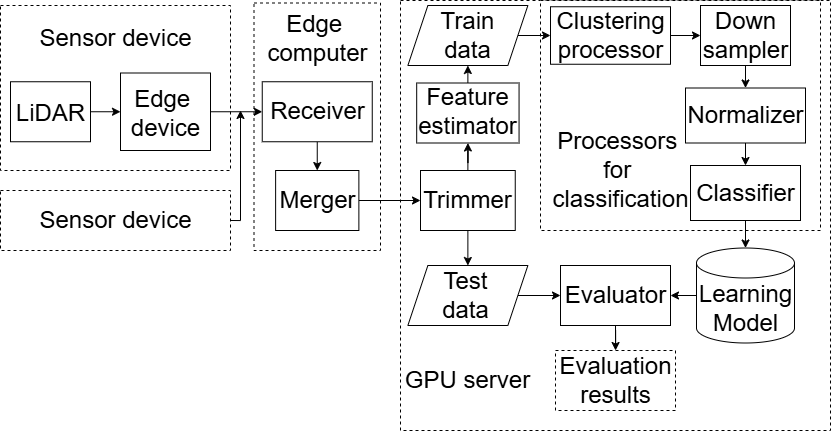
\includegraphics[width=\linewidth]{img/journal_system8.drawio.png}}
  \caption{System model.}
  \label{system}
\end{figure}


\subsection{Methodology}
\label{sec:method}
% \begin{spverbatim}
%1st paragraph
%1
\revised{3D data is acquired using the system presented by Akiyama et al. and Li et al. \cite{9789786,9507455}.}
\deleted{In the proposed system, 3D data is acquired using the system presented by Akiyama et al. and Li et al. \cite{9789786,9507455}.}
  %1-1
  \revised{Multiple LiDAR calibrations merge streams by rotating and translating 3D data according to predetermined angles and distances.}
  \begin{deletedblock}
  Multiple LiDAR calibrations are performed for merging and the angles and distances are determined. 
    The axis of the 3D data is rotated based on the angles, and the 3D data is translated based on the distances.
  \end{deletedblock}

%2nd paragraph
%2
The point cloud of each frame of the aggregated 3D data is trimmed.
  %2-1
  \revised{Vertices of each person's region are determined manually under a fixed-seating office layout.}
  \begin{deletedblock}
  Here, the coordinates of the vertices of a region where a person is located are determined manually, and the region is cut out. 
    The manual determination assumes a fixed-seating office environment, where the location of each person's workspace is pre-determined and known in advance.
  \end{deletedblock}

%3rd paragraph
%3
\revised{Four feature types were selected to capture complementary geometric properties of hand-region point clouds.}
  %3-1
  \revised{Normals encode local surface orientation of hands and forearms.}
  %3-2
  \revised{Dimensionality features distinguish linear, planar, and volumetric local structures.}
  %3-3
  \revised{Proportion of variance summarizes eigenvalue distribution within each neighborhood.}
  %3-4
  \revised{FPFH encodes pairwise angular relationships among neighboring points.}
%4
Four types of features are extracted from the trimmed point clouds: normals, dimensionality features, proportion of variance, and FPFH. 
  %4-1
  \revised{For normals, dimensionality features, and proportion of variance, the k-nearest neighbor algorithm (KNN) uses search radius 100 and maximum 30 neighbors to build covariance matrices at each point.}
  \deleted{The k-nearest neighbor algorithm (KNN) is implemented using the determined parameters.}
  %4-2
  \textit{Normals.} 
    %4-2-1
    \revised{Eigenvectors of the smallest eigenvalue in each covariance matrix serve as normals (Fig.~\ref{features}\subref{normal}).}
    \begin{deletedblock}
      The search radius was 100. 
      The maximum number of neighbors was 30. 
    Covariance matrices are generated from each point in the point cloud based on KNN. 
    Eigenvectors corresponding to the smallest eigenvalue in the covariance matrices are used as the normals. 
    Fig.~\ref{features}\subref{normal} shows the data with the normals. 
    \end{deletedblock}
  %4-3
  \textit{Dimensionality features} \cite{isprs-archives-XXXVIII-5-W12-97-2011,YANG201319}.
    %4-3-1
    \revised{Eigenvalues ${\lambda}_i$, $i=[1, 3]$ yield $a_{1D}=\frac{\sqrt{{\lambda}_1}-\sqrt{{\lambda}_2}}{\sqrt{{\lambda}_1}}$, $a_{2D}=\frac{\sqrt{{\lambda}_2}-\sqrt{{\lambda}_3}}{\sqrt{{\lambda}_1}}$, and $a_{3D}=\frac{\sqrt{{\lambda}_3}}{\sqrt{{\lambda}_1}}$ \cite{isprs-archives-XXXVIII-5-W12-97-2011,YANG201319} (Fig.~\ref{features}\subref{dimensionality}).}
    \begin{deletedblock}
    KNN is performed using the determined parameters. 
    Covariance matrices are generated from each point in the point cloud based on KNN. 
    Eigenvalues are defined as ${\lambda}_i$, $i=[1, 3]$ and the dimensionality features are calculated as $a_{1D}=\frac{\sqrt{{\lambda}_1}-\sqrt{{\lambda}_2}}{\sqrt{{\lambda}_1}}$, $a_{2D}=\frac{\sqrt{{\lambda}_2}-\sqrt{{\lambda}_3}}{\sqrt{{\lambda}_1}}$, and $a_{3D}=\frac{\sqrt{{\lambda}_3}}{\sqrt{{\lambda}_1}}$\cite{isprs-archives-XXXVIII-5-W12-97-2011,YANG201319}. 
    Fig.~\ref{features}\subref{dimensionality} shows the data with the dimensionality features. 
    \end{deletedblock}
  %4-4
  \textit{Proportion of variance} \cite{BRODU2012121}. 
    %4-4-1
    \revised{Proportion of variance is $\boldsymbol{v_i}=\frac{{\lambda}_i}{{\lambda}_1+{\lambda}_2+{\lambda}_3}(i=[1, 3])$ (Fig.~\ref{features}\subref{proportion}).}
    \begin{deletedblock}
    KNN is performed using the determined parameters. 
    Covariance matrices are generated from each point in the point cloud based on the KNN. 
    Eigenvalues are defined as ${\lambda}_i$, $i=[1, 3]$ and the proportion of variance is calculated as $\boldsymbol{v_i}=\frac{{\lambda}_i}{{\lambda}_1+{\lambda}_2+{\lambda}_3}(i=[1, 3])$. 
    Fig.~\ref{features}\subref{proportion} shows the data with the proportion of variance. 
    \end{deletedblock}
  %4-5
  \textit{FPFH} \cite{5152473}. 
    %4-5-1
    \revised{Two adjacent points per center point define a Darboux frame; FPFH is computed from frame-based angular relations and concatenated; principal component analysis (PCA) with randomized singular value decomposition reduces the 33-dimensional FPFH to three dimensions (Fig.~\ref{features}\subref{fpfh}).}
    \begin{deletedblock}
    Two points in a set of points adjacent to each point in the point cloud are chosen on the basis of the parameters \cite{4795593,4650967}. 
    The Darboux frame $u$, $v$, and $w$ are defined by using the two points and normals. 
    Three variables are defined. 
      The first variable is a dot product vector between the one of the normal and the frame $v$. 
      The second variable is a unit vector of a dot product vector between the one of a distance vector of two points and the frame $v$. 
      The third variable is an arctangent function consisting of a dot product vector between the one of the normal and the frame $u$, and a dot product vector between the one of the normal and the frame $w$. 
      The FPFH is generated from combinations of a center point and the surrounding points in the point cloud and then several FPFHs are concatenated. 
    PCA is used to reduce the dimensions of the FPFH. 
      PCA is used to reduce the 33-dimensional FPFH to three dimensions.
      The randomized SVD solver is used. 
    Fig.~\ref{features}\subref{fpfh} shows the data with the FPFH. 
    \end{deletedblock}

%4th paragraph
%5
Next, clustering is performed for the point clouds using the point features. 
  %5-1
  \revised{DBSCAN ($\varepsilon=100$, minimum 10 points on 3D coordinates) and k-means ($k=3$) each remove outliers and extraneous clusters \cite{ester1996density,hartigan1979algorithm}.}
  %5-2
  \revised{DBSCAN removes isolated noise points from background objects and sensor reflections.}
  %5-3
  \revised{k-means partitions the point cloud into fixed spatial groups; extraneous partitions are discarded.}
  %5-4
  \revised{Aggressive cluster removal can delete sparse finger points and degrade classification of fine hand postures.}
  \begin{deletedblock}
  DBSCAN is used to determine the parameters for DBSCAN so as to remove noise in the point cloud and then align circles to each point in the point cloud on the basis of the parameters \cite{ester1996density}.
      The neighborhood radius $\varepsilon$ is 100. 
      The minimum number of points is 10. 
      DBSCAN is applied to the three-dimensional coordinates of each point. 
    Points that have more than a certain number of points in the circle centered at the point are defined as ``core'' and points within the radii of the circles that the cores have are defined as ``reachable points''. 
    Points that are not near to any cores are considered outliers. 
    The outliers and some of the clusters are removed. 
  k-means is used to determine the number of clusters for k-means so as to remove noise in the point cloud \cite{hartigan1979algorithm}. 
    The number of clusters $k$ was 3.
    Each point in the point cloud is randomly assigned to a cluster, and as long as the cluster changes, the following process is repeated. 
      Specifically, the centroids of each cluster are determined and the cluster to which each point belongs is changed in accordance with the nearest center of the centroids. 
    The outliers and some of the clusters are removed. 
  \end{deletedblock}

%5th paragraph
%6
Downsampling is performed for the clustered point clouds. 

%6th paragraph
%7
\revised{Downsampled training point clouds are normalized so that the distance from the center of gravity to the farthest point equals 1.0.}
\begin{deletedblock}
Normalization is performed for the downsampled point clouds for the training data. 
  Here, 1.0 is set as the distance from the center of gravity to the farthest point. 
  The downsampled point clouds are normalized on the basis of this distance. 
\end{deletedblock}

%7th paragraph
%8
\revised{PointNet++ classifies normalized point clouds by repeatedly selecting points, grouping neighborhoods, and processing each group with PointNet and a fully connected layer \cite{DBLP:journals/corr/QiYSG17}.}
  %8-1
  \revised{Two-level grouping in PointNet++ captures hand-scale local structures that distinguish mouse operation, pad operation, typing, and sitting still.}
\deleted{Classification is performed for the normalized point clouds utilizing PointNet++ to determine the parameters for PointNet++ so as to determine size of the data to process \cite{DBLP:journals/corr/QiYSG17}.}
  \deleted{The following process is repeated twice: a few points in each point cloud are first chosen, a group formed from each selected point and the surrounding points is created, and then each group is processed using PointNet and a fully connected layer.}

% \end{spverbatim}
%6/27 tb ⇒ t
\begin{deletedblock}
\begin{figure}[t]
  \centering
  {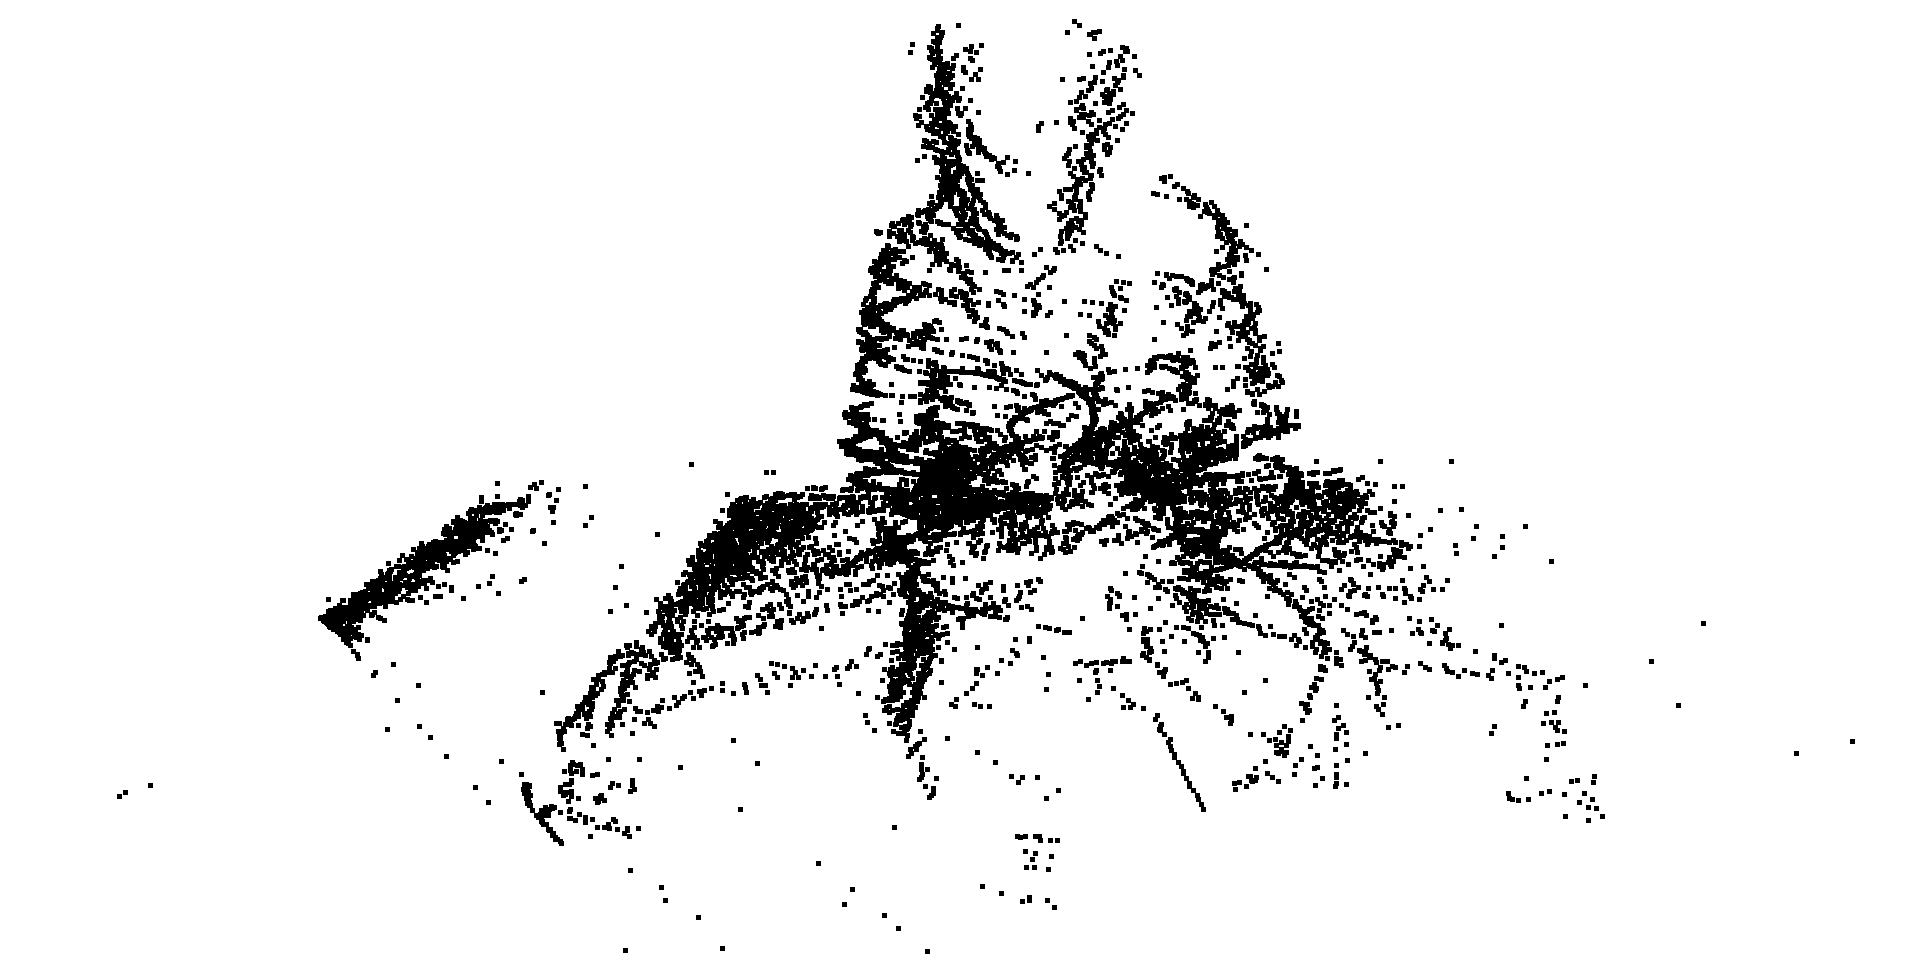
\includegraphics[width=\linewidth]{img/cutdata.png}}
  \caption{Trimmed data.}
  \label{trimdata}
\end{figure}
\end{deletedblock}

%6/27 tb ⇒ t
\begin{figure}[t]
  \centering
  \subfloat[Normals]{
    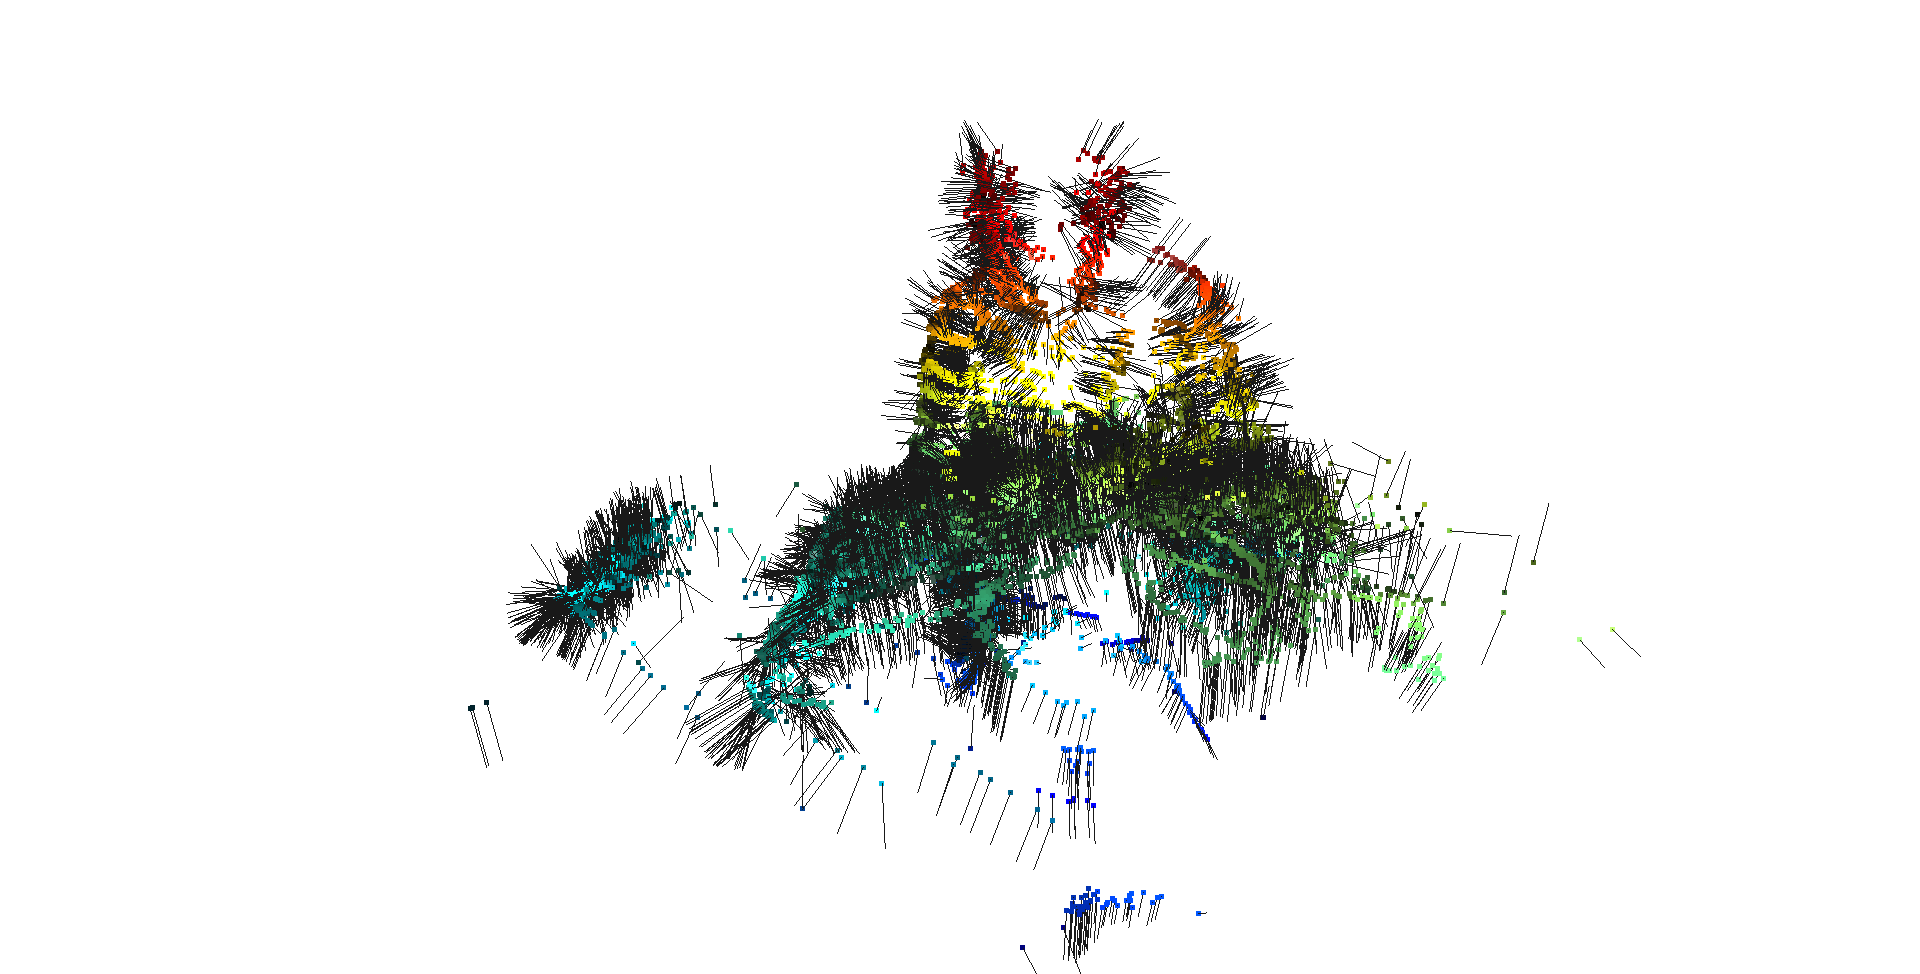
\includegraphics[width=.45\linewidth]{img/normal.png}
    \label{normal}
  }
  \subfloat[Dimensionality features]{
    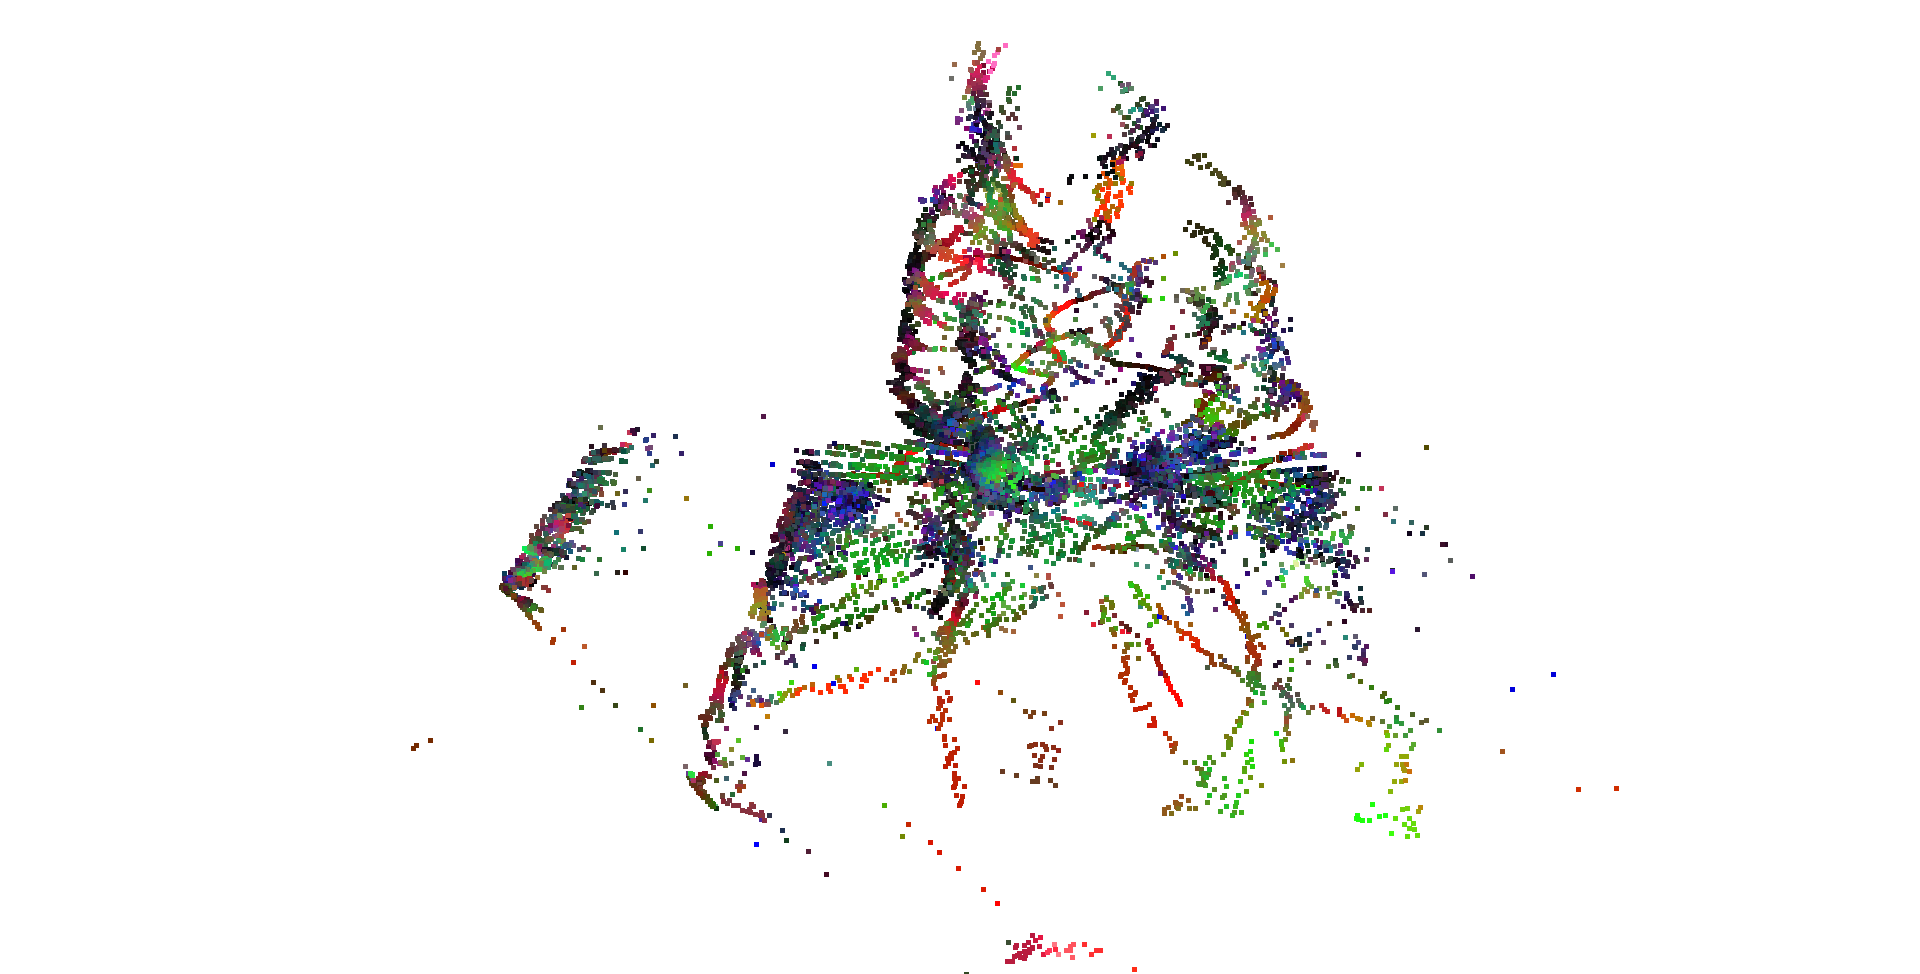
\includegraphics[width=.45\linewidth]{img/dim.png}
    \label{dimensionality}
  }
  \\
  \subfloat[Proportion of variances]{
    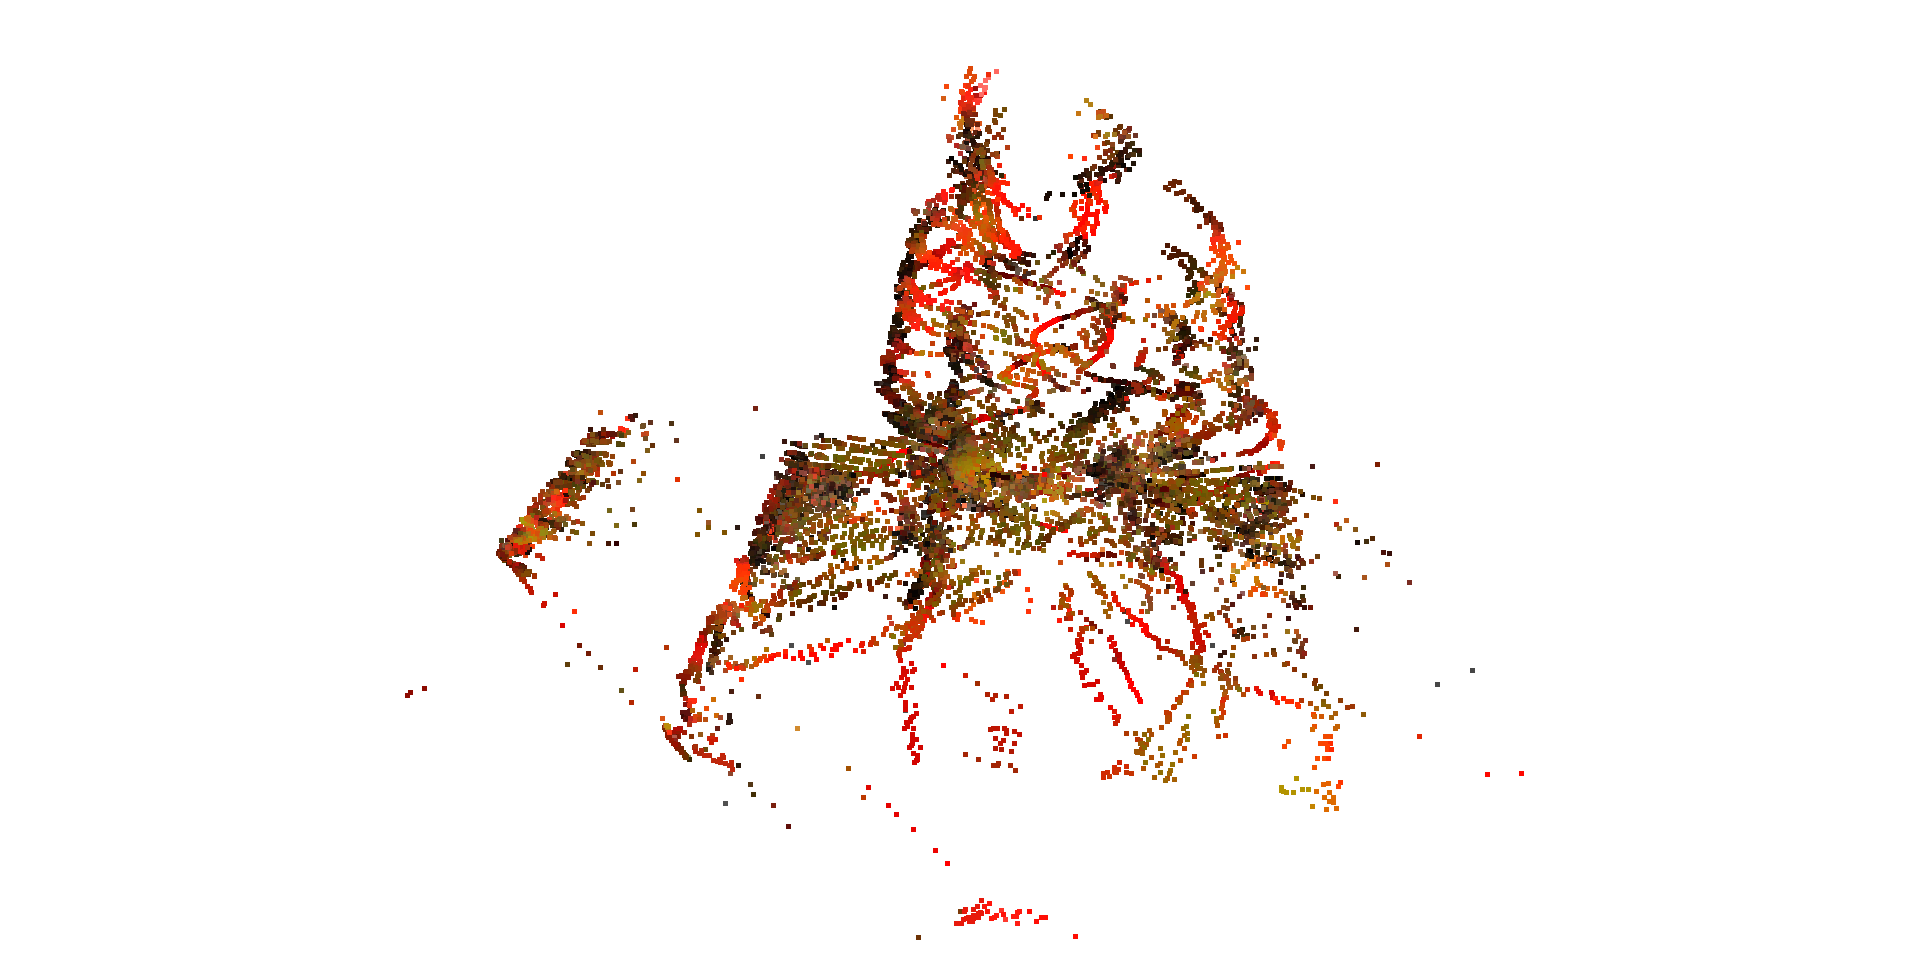
\includegraphics[width=.45\linewidth]{img/proportion.png}
    \label{proportion}
  }
  \subfloat[FPFH]{
    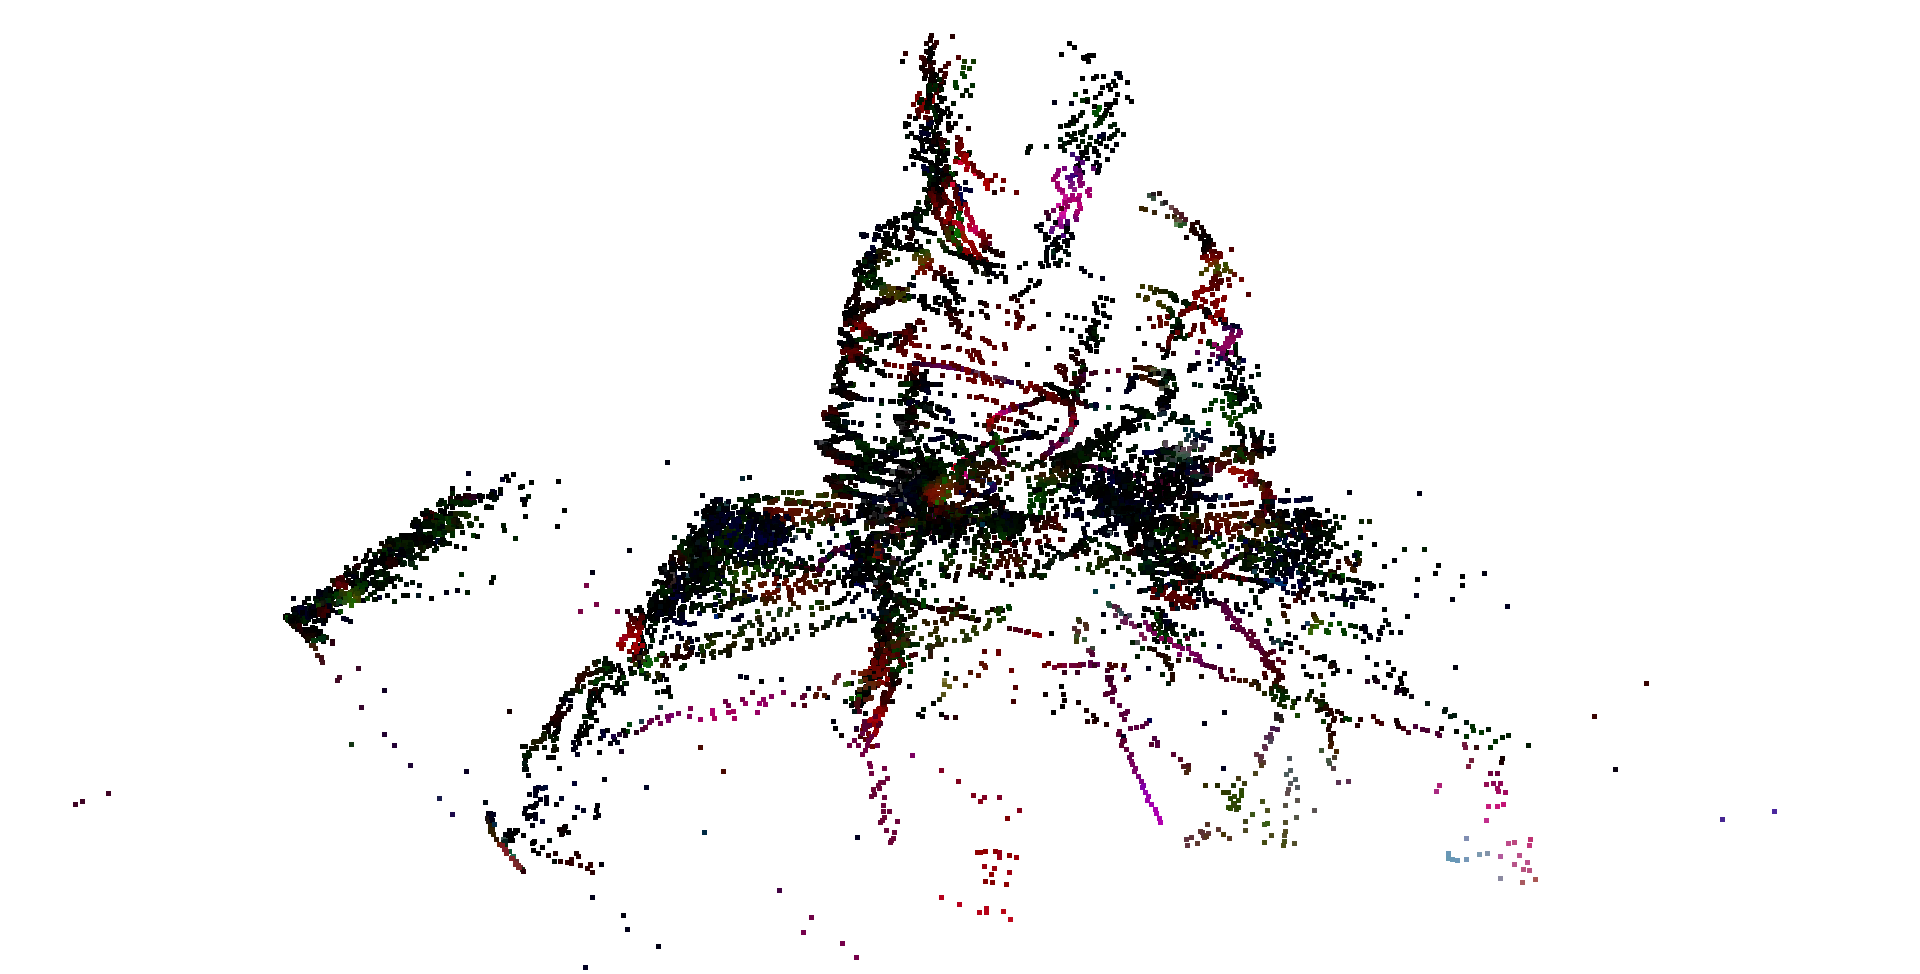
\includegraphics[width=.45\linewidth]{img/fpfh.png}
    \label{fpfh}
  }
  \caption{Point clouds with each of four types of feature.}
  \label{features}
\end{figure}


\section{Experiment setup}
\label{sec:experiment}
\subsection{Experimental system}
% \begin{spverbatim}
%1st paragraph
%1
\revised{An experimental system was built from the model in Fig.~\ref{system}.}
\deleted{We developed an experimental system based on the proposed system shown in Fig.~\ref{system}.}
%2
The experimental system consisted of two sets of LiDAR units (Mid-70 units), two edge devices (Jetson nano units), an edge computer (Jetson Xavier NX and Jetson Orin nano), and a regular keyboard \cite{Mid70,Jetsonnano,JetsonNX,Jetsonorinnano}.
  %2-1
  \revised{The experiment was conducted at 14Q32, 14F, Shibaura Institute of Technology, Toyosu, Koto-ku, Tokyo.}
  %2-2
  \revised{Two Livox Mid-70 LiDAR units were deployed at a sensor frame rate of 10 fps.}
  %2-3
  \revised{Two NVIDIA Jetson nano edge devices were used.}
  %2-4
  \deleted{An NVIDIA Jetson Xavier NX edge computer was used for training data and test data A, B, and C acquisition.}
  \revised{An NVIDIA Jetson Xavier NX edge computer was used for training data and test data acquisition on 9 December 2022.}
  %2-5
  \deleted{An NVIDIA Jetson Orin nano edge computer was used for test data A to AB acquisition.}
  \revised{An NVIDIA Jetson Orin nano edge computer was used for test data acquisition on 12 December 2024.}
\deleted{Table~\ref{experiment} lists the specifications of the experiment.}

%2nd paragraph
%3
\deleted{Training data and test data A, B, and C were acquired on 9 December 2022.}
\revised{Training data and test data were acquired on 9 December 2022.}
%4
\deleted{Test data A to AB were acquired on 12 December 2024.}
\revised{Test data were acquired on 12 December 2024.}
%5
\deleted{3 contributors provided training data.}
\deleted{3 experiment participants provided training data.}
%6
\deleted{28 contributors provided test data.}
\deleted{28 experiment participants provided test data.}

\begin{deletedblock}
\begin{table}[b]
	\caption{Specifications of experiment.}
	\label{experiment}
    \scalebox{0.9}{
	\begin{tabular}{l|l}
        \hline
        Parameter & Value \\ \hline
        Place & 14Q32, 14F, Shibaura Institute \\
        &of Technology, Toyosu, Koto-ku, \\ 
        &Tokyo \\
        Date of training data \\
        and test data A, B, \\
        and C acquisition & 9 December 2022 \\
        Date of test data \\
        A to AB acquisition & 12 December 2024 \\
        LiDAR units & Livox Mid-70 \\
        No. of LiDAR units & 2 \\
        Edge devices & NVIDIA Jetson nano \\
        No. of edge devices & 2 \\
        Edge computer for training data \\ 
        and test data A, B, \\
        and C acquisition & NVIDIA Jetson Xavier NX \\
        Edge computer for test data \\ 
        A to AB acquisition & NVIDIA Jetson Orin nano \\
        Frame rate of sensor & 10 fps \\
        No. of contributors for training data & 3 \\
        No. of contributors for test data & 28 \\
        \hline
 \end{tabular}
 }
\end{table}
\end{deletedblock}
% \end{spverbatim}


\subsection{LiDAR deployment}
% \begin{spverbatim}
%1LiDAR配置の図
\deleted{Fig.~\ref{jlidar} shows the deployment of the devices for the experiment.}
%2具体的な配置方法
%blue
The two LiDAR sensors were placed on a table facing each other.
\deleted{They were positioned 1.0 m away from the subject in a lateral direction and tilted down by $10^{\circ}$ to make the PC easier to detect.}
\revised{They were positioned 1.0 m away from the experiment participant in a lateral direction and tilted down by $10^{\circ}$ to make the PC easier to detect.}
\deleted{The PC was placed on the table in front of the subject.}
\revised{The PC was placed on the table in front of the experiment participant.} 
%3実験の様子
Fig.~\ref{experimentsite} shows the experiment site. 
  
% \end{spverbatim}

\begin{figure}[t]
  \centering
  {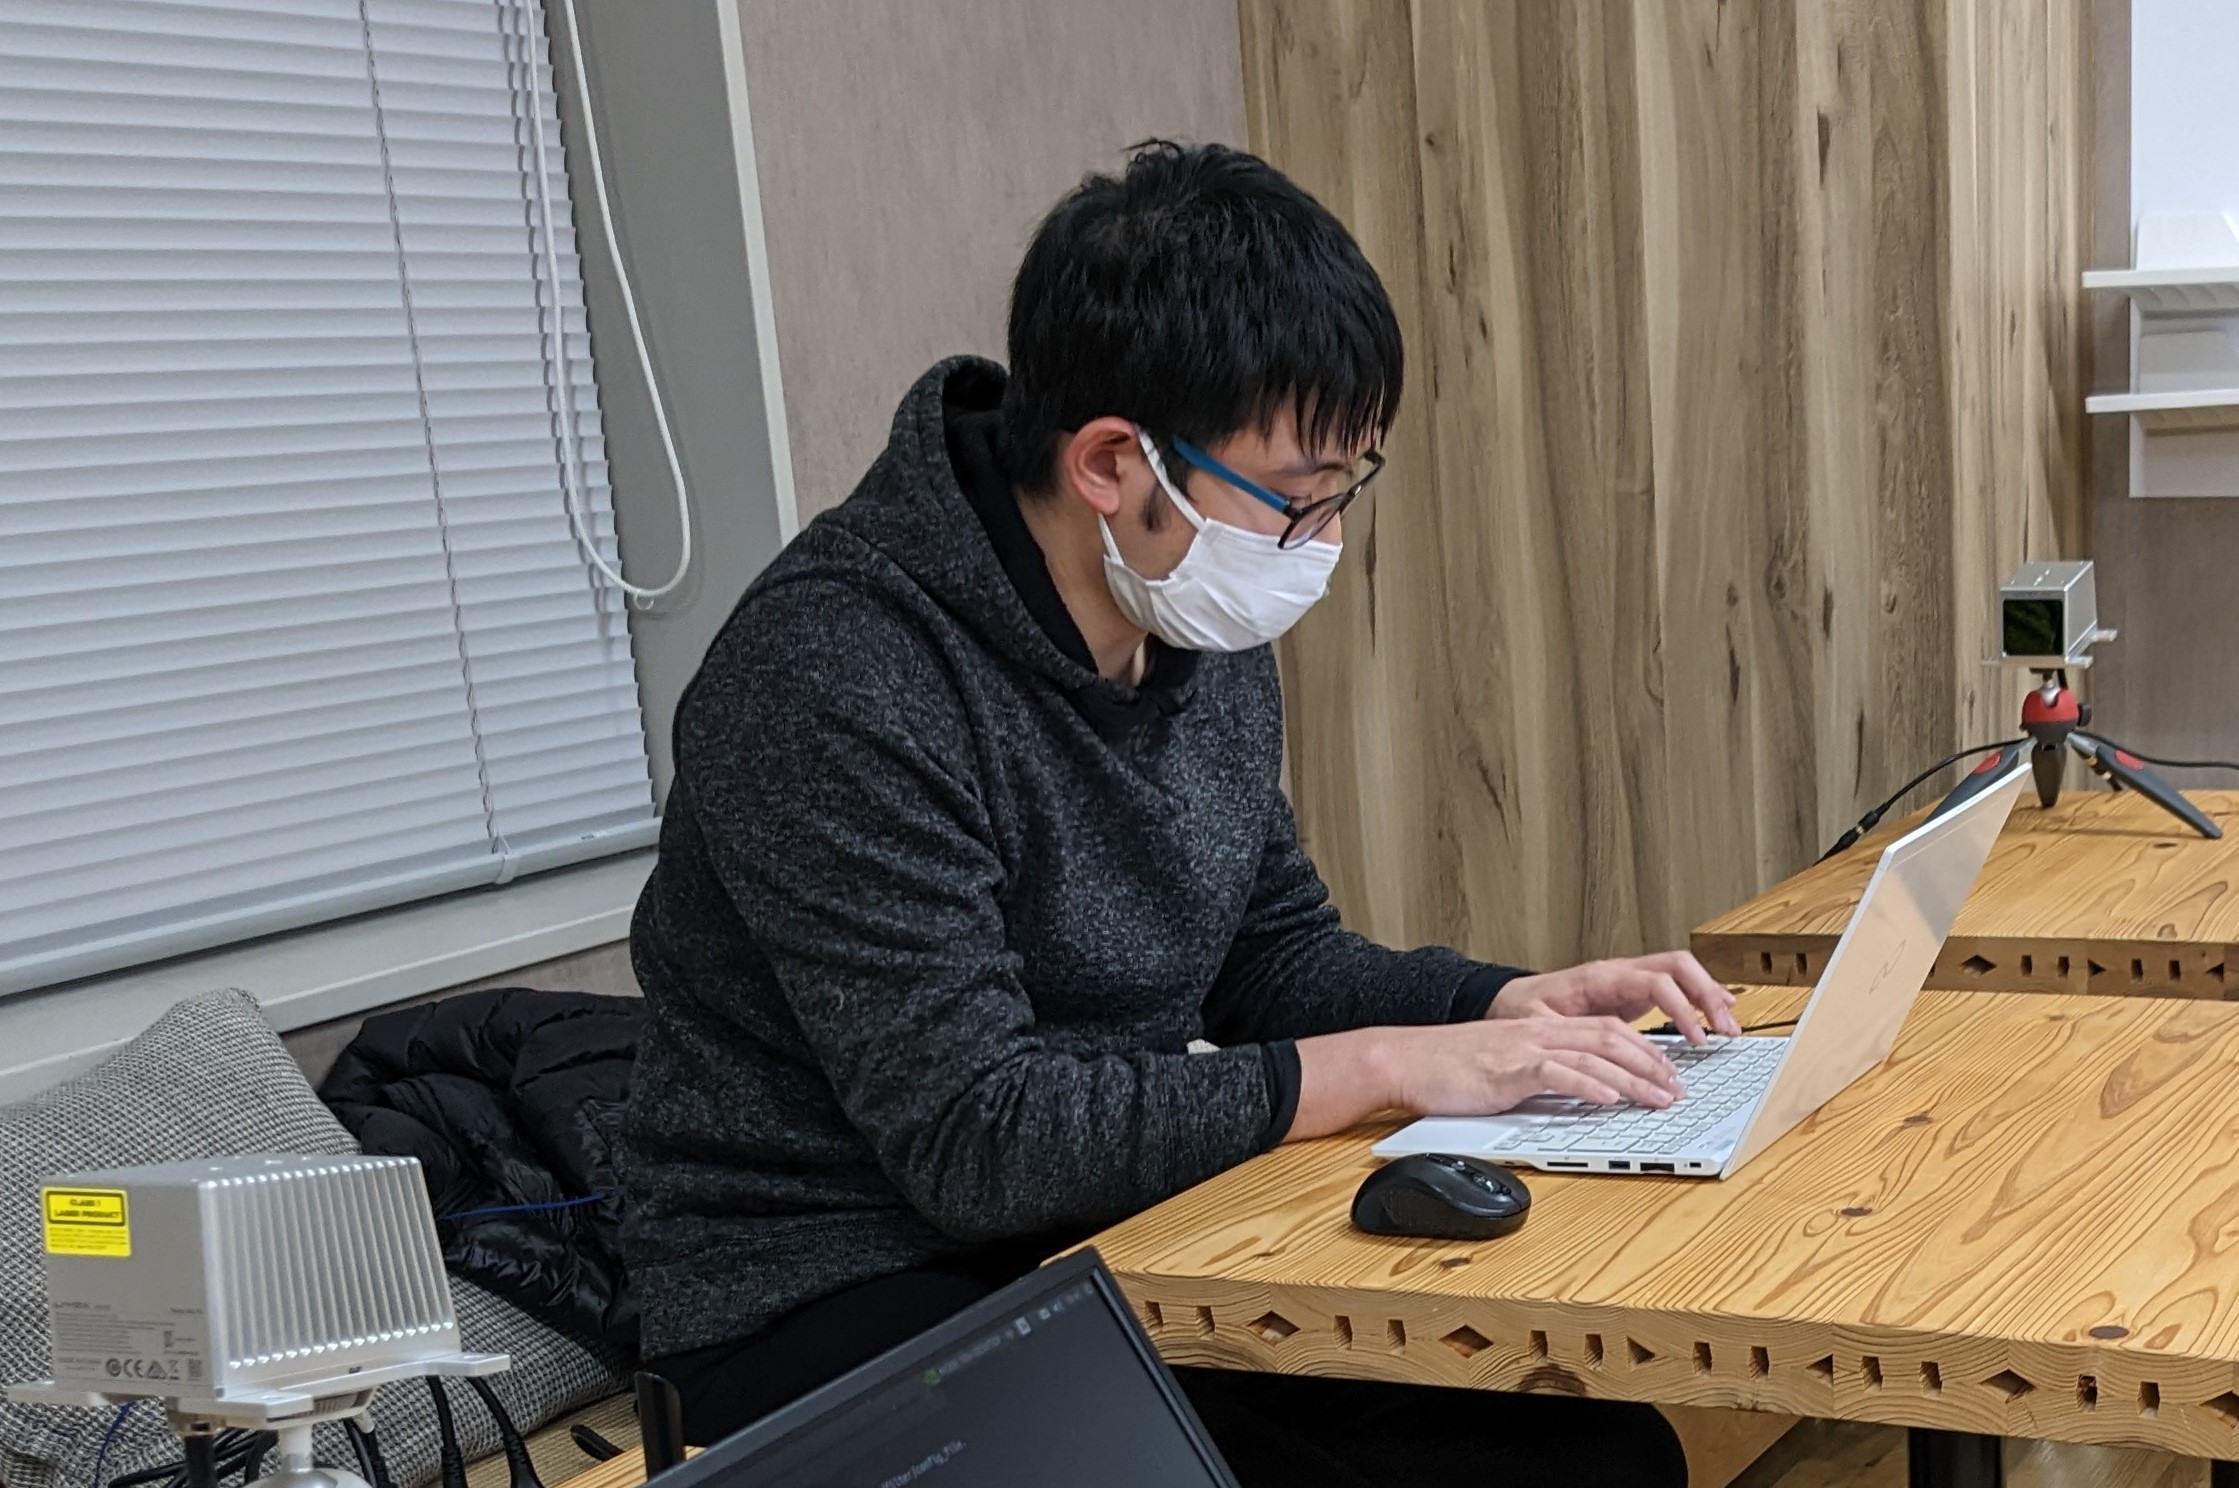
\includegraphics[width=\linewidth]{img/experimentsite2.jpg}}
  \caption{Experiment site.}
  \label{experimentsite}
\end{figure}

\begin{deletedblock}
\begin{figure}[t]
  \centering
  {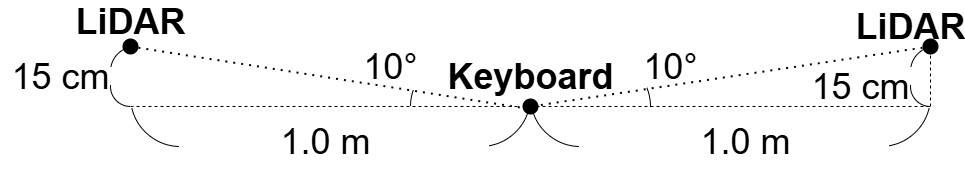
\includegraphics[width=\linewidth]{img/ld_journal5.drawio.png}}
  \caption{Deployment of LiDAR sensors.}
  \label{jlidar}
\end{figure}
\end{deletedblock}

\subsection{Data acquisition}
\subsubsection{Training data acquisition}
%1 協力者31名の選定
\begin{revisedblock}
We selected 31 experiment participants.
  %1-1 年齢帯
  The 31 experiment participants were in their 20s.
  %1-2 日常的なPC利用
  The 31 experiment participants used a PC daily.
\end{revisedblock}

%2トレーニングデータの取得方法
\deleted{LiDAR was used to acquire training data on the subject's posture while using the PC to perform four tasks.}
\revised{LiDAR was used to acquire training data on the experiment participant's posture while using the PC to perform four tasks.}\footnote{Our experiment was approved by the Ethics Committee of Shibaura Institute of Technology.}

\revised{Table~\ref{dataacquisition} summarizes data acquisition conditions for training data; each capture was repeated 20 times for mouse operation, pad operation, and typing, and 10 times for sitting still.}
\deleted{Table~\ref{trainacquisition} summarizes training data acquisition conditions; each capture was repeated 20 times for mouse operation, pad operation, and typing, and 10 times for sitting still.}
\begin{deletedblock}
As for mouse operation, the posture of the subjects was captured for 30 seconds as they manipulated a mouse to write the alphabet in order from ``A'' to ``Z''. The capturing was repeated 20 times to acquire training data. 
    Fig.~\ref{labels}\subref{pcmouse} shows the point cloud of the mouse operation. 
As for pad operation, the posture of the subjects was captured for 30 seconds as they performed a pad operation on the PC to write the alphabet in order from ``A'' to ``Z''. The capturing was repeated 20 times to acquire training data. 
    Fig.~\ref{labels}\subref{pcpad} shows the point cloud of the pad operation. 
As for sitting still, the posture of the subjects was captured for ten  seconds as they sat still without moving and did not touch the PC. The capturing was repeated ten times to acquire training data. 
    Fig.~\ref{labels}\subref{pcstay} shows the point cloud of sitting still. 
As for typing, the posture of the subjects was captured for 30 seconds as they typed the alphabet in order from ``A'' to ``Z''. The capturing was repeated 20 times to acquire training data. 
    Fig.~\ref{labels}\subref{pctyp} shows the point cloud of the typing. 
\end{deletedblock}

\begin{revisedblock}
\begin{table}[b]
  \centering
  \revised{\caption{Data acquisition conditions for each posture class.}}
  \deleted{\caption{Training data acquisition conditions for each posture class.}}
  \label{dataacquisition}
  \scalebox{0.9}{
  \begin{tabular}{l|l|c}
    \hline
    Posture class & Task & Duration \\ \hline
    Mouse operation & Write alphabet A--Z using mouse & 30 s \\
    Pad operation & Write alphabet A--Z using trackpad & 30 s \\
    Sitting still & Sit still without moving or touching PC & 10 s \\
    Typing & Type alphabet A--Z on keyboard & 30 s \\
    \hline
  \end{tabular}
  }
\end{table}
\end{revisedblock}

\revised{Fig.~\ref{labels} shows point clouds for each posture class.}

%6トレーニングデータの被験者
\revised{We randomly sampled three experiment participants from the 31 experiment participants.}
\deleted{The three subjects in this study are denoted as subjects A, B, and C.}
\revised{The three experiment participants in this study are denoted as experiment participants A, B, and C.}
    % Training data with subjects A, B, and C is called training data A, B, and C, and test data with subjects A, B, and C is called test data A, B, and C. 
    %6-1トレーニングデータの名称
    \deleted{Training data with subjects A, B, and C is called training data A, B, and C.}
    \revised{Training data with experiment participants A, B, and C is called training data A, B, and C.} 

\subsubsection{Test data acquisition}
%1テストデータについて
\begin{deletedblock}
Test data were acquired for the four types of postures: mouse operation, pad operation, sitting still, and typing, as for training data. 
As for mouse operation, the posture of the subjects was captured for 30 seconds as they manipulated a mouse to write the alphabet in order from ``A'' to ``Z''. The capturing was performed only once to acquire test data.
As for pad operation, the posture of the subjects was captured for 30 seconds as they performed a pad operation on the PC to write the alphabet in order from ``A'' to ``Z''. The capturing was performed only once to acquire test data. 
As for sitting still, the posture of the subjects was captured for ten seconds as they sat still without moving and did not touch the PC. The capturing was performed only once to acquire test data. 
As for typing, the posture of the subjects was captured for 30 seconds as they typed the alphabet in order from ``A'' to ``Z''. The capturing was performed only once to acquire test data.
\end{deletedblock}

\deleted{Test data were acquired for the four posture classes under the conditions summarized in Table~\ref{dataacquisition}; each capture was performed once per subject.}
\revised{Test data were acquired for the four posture classes under the conditions summarized in Table~\ref{dataacquisition}; each capture was performed once per experiment participant.}
\deleted{Test data were acquired for the four posture classes under the conditions summarized in Table~\ref{testacquisition}; each capture was performed once per subject.}
\begin{deletedblock}
\begin{table}[b]
  \centering
  \caption{Test data acquisition conditions for each posture class.}
  \label{testacquisition}
  \scalebox{0.9}{
  \begin{tabular}{l|l|c}
    \hline
    Posture class & Task & Duration \\ \hline
    Mouse operation & Write alphabet A--Z using mouse & 30 s \\
    Pad operation & Write alphabet A--Z using trackpad & 30 s \\
    Sitting still & Sit still without moving or touching PC & 10 s \\
    Typing & Type alphabet A--Z on keyboard & 30 s \\
    \hline
  \end{tabular}
  }
\end{table}
\end{deletedblock}

%6テストデータの被験者
\revised{We used 28 experiment participants from the 31 experiment participants.}
  \revised{The 28 experiment participants were not sampled for training.}
\deleted{The 28 subjects in this study are denoted as subjects A to AB.}
\revised{The 28 experiment participants in this study are denoted as experiment participants A to AB.}
    %6-1テストデータの名称（データセット別名は削除）
    \deleted{Test data with subjects A to AB is called test data A to AB.}
    \deleted{Test data with experiment participants A to AB is called test data A to AB.}

% \end{spverbatim}
 
% \begin{figure}[ht]
%   \centering
%   \subfloat[Left LiDAR sensor]{
%     \includegraphics[width=.6\linewidth]{img/pcleft.png}
%     \label{pcleft}
%   }
%   \\
%   \subfloat[Right LiDAR sensor]{
%     \includegraphics[width=.6\linewidth]{img/pcright.png}
%     \label{pcright}
%   }
%   \\
%   \subfloat[Both LiDAR sensors]{
%     \includegraphics[width=.6\linewidth]{img/pcmerge.png}
%     \label{pcmerged}
%   }
%   \caption{Visualization of data from each LiDAR.}
%   \label{eachlidar}
% \end{figure} 
 
%6/27 tb ⇒ t
\begin{figure}[t]
  \centering
  \subfloat[Mouse operation]{
    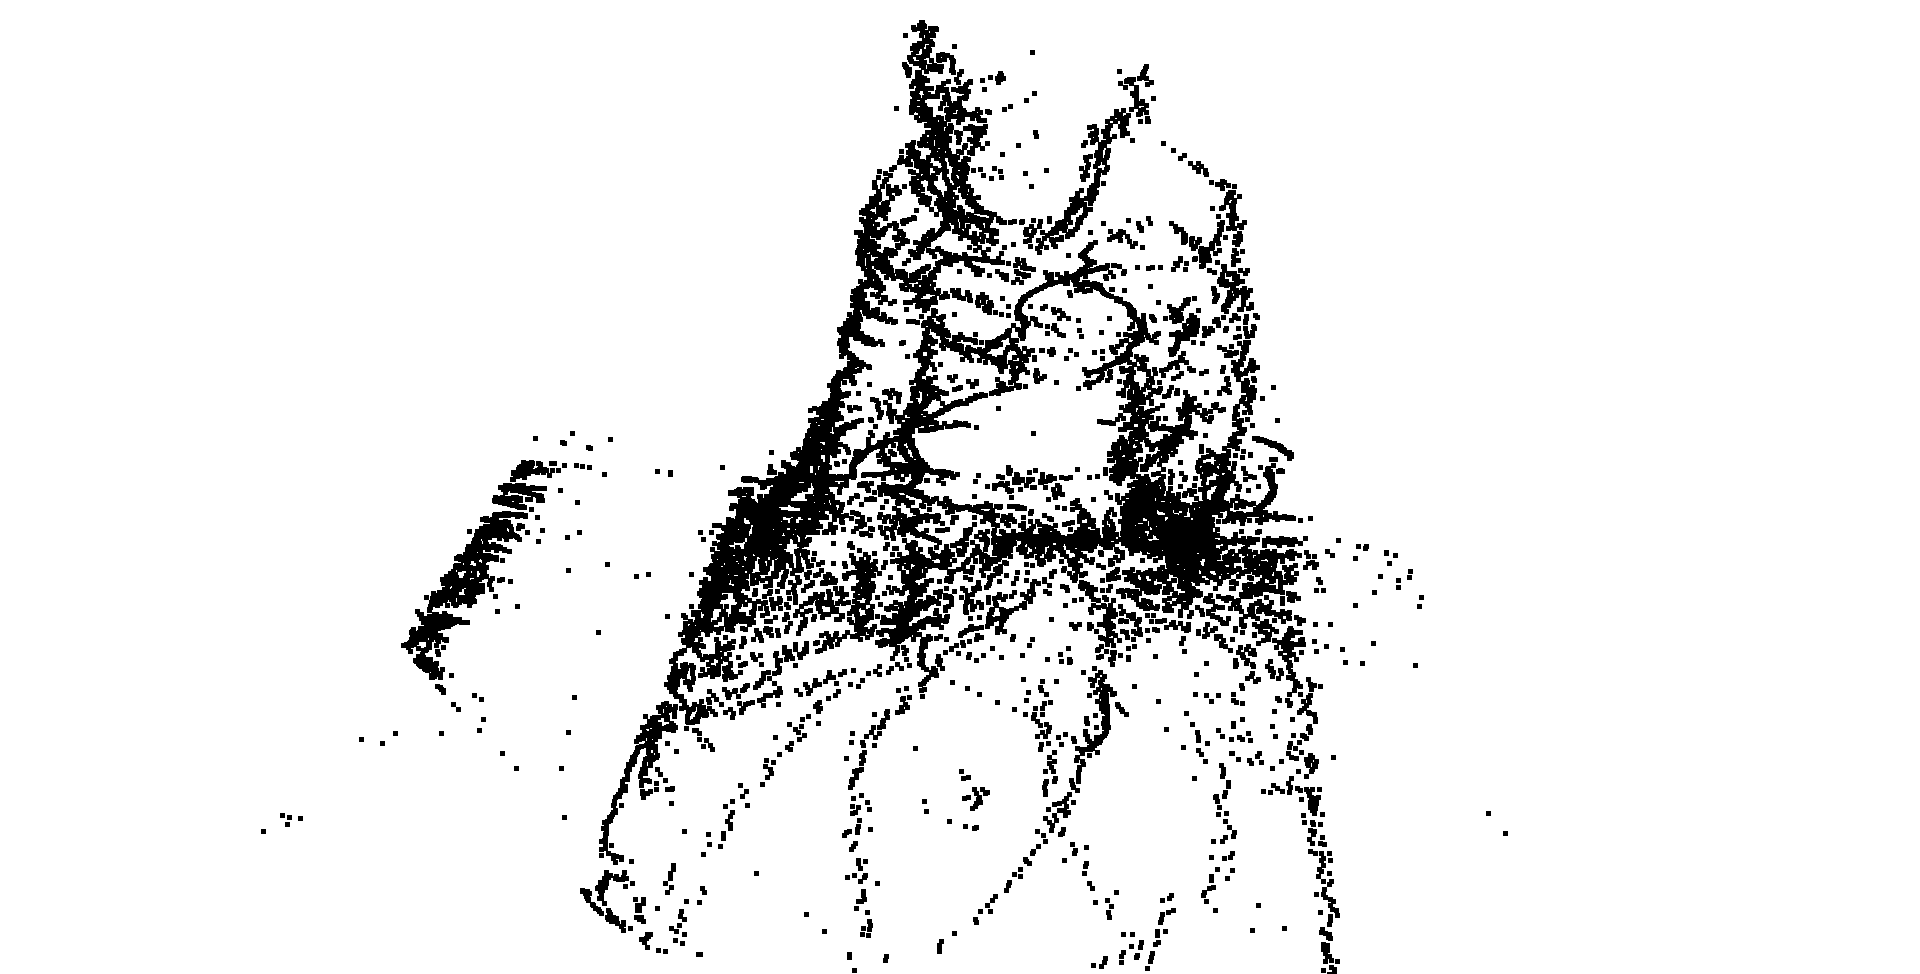
\includegraphics[width=.45\linewidth]{img/mouse.png}
    \label{pcmouse}
  }
  \subfloat[Pad operation]{
    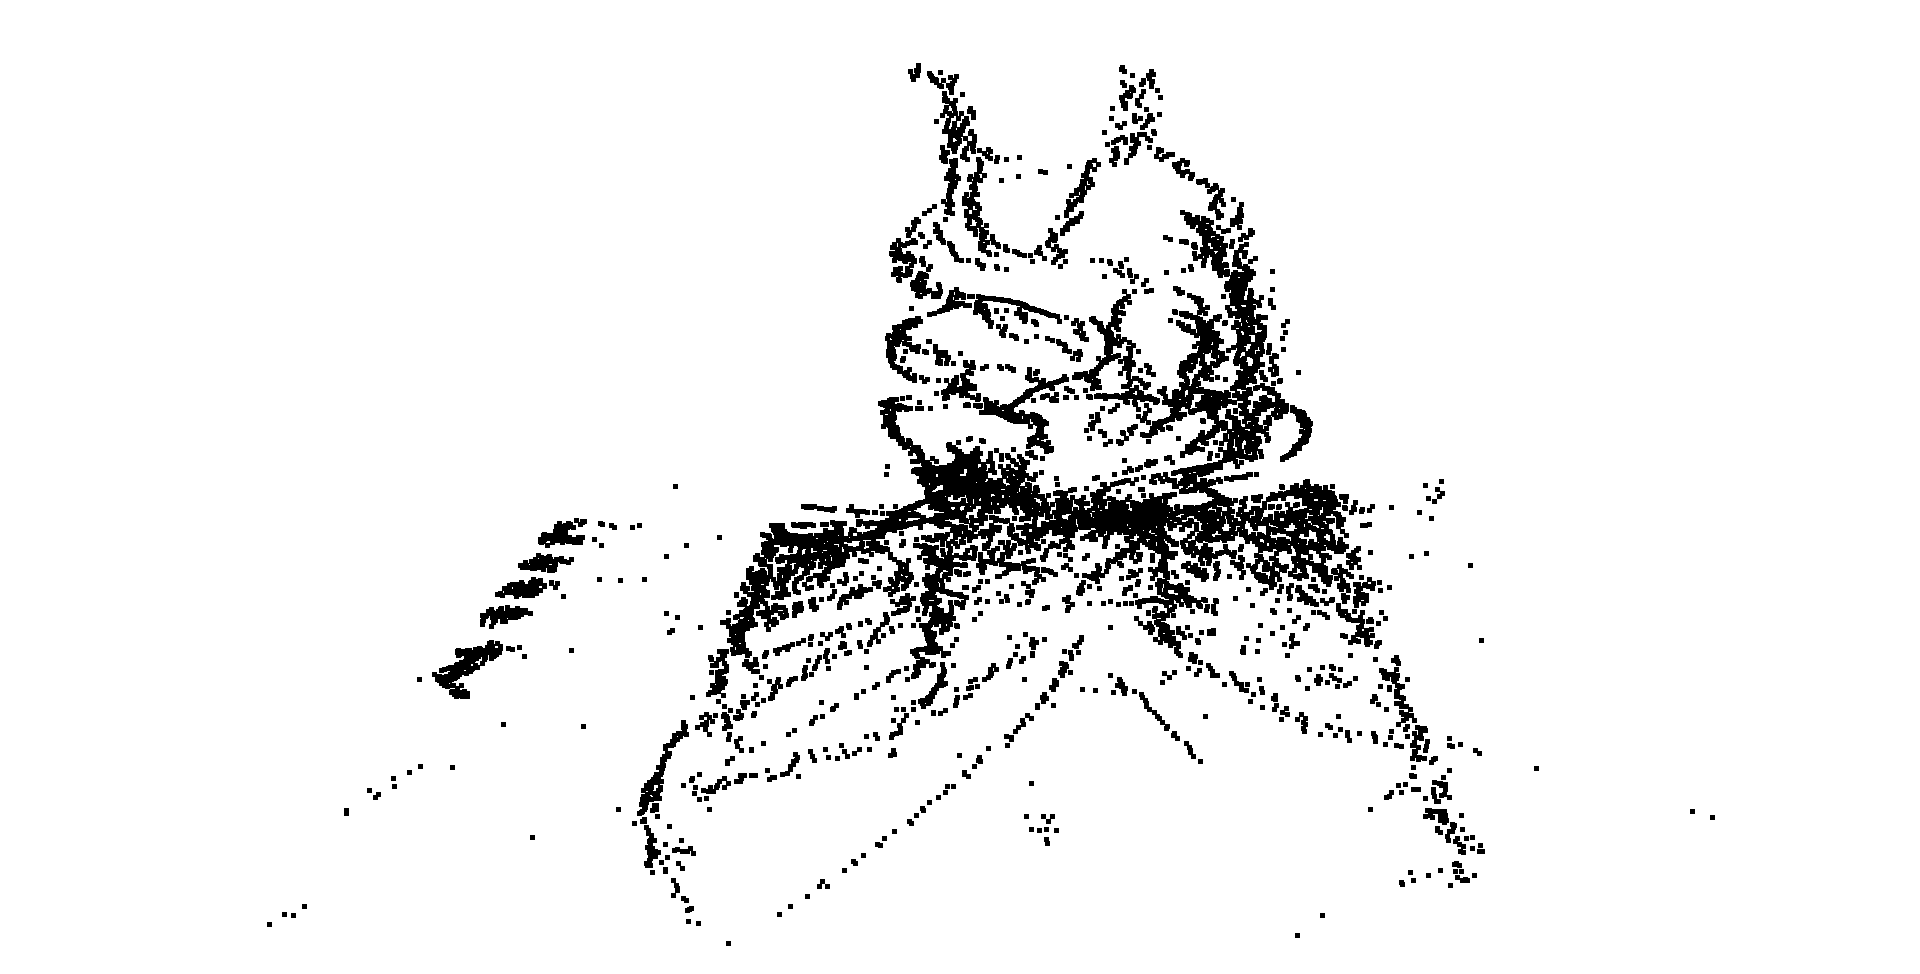
\includegraphics[width=.45\linewidth]{img/pat.png}
    \label{pcpad}
  }
  \\
  \subfloat[Sitting still]{
    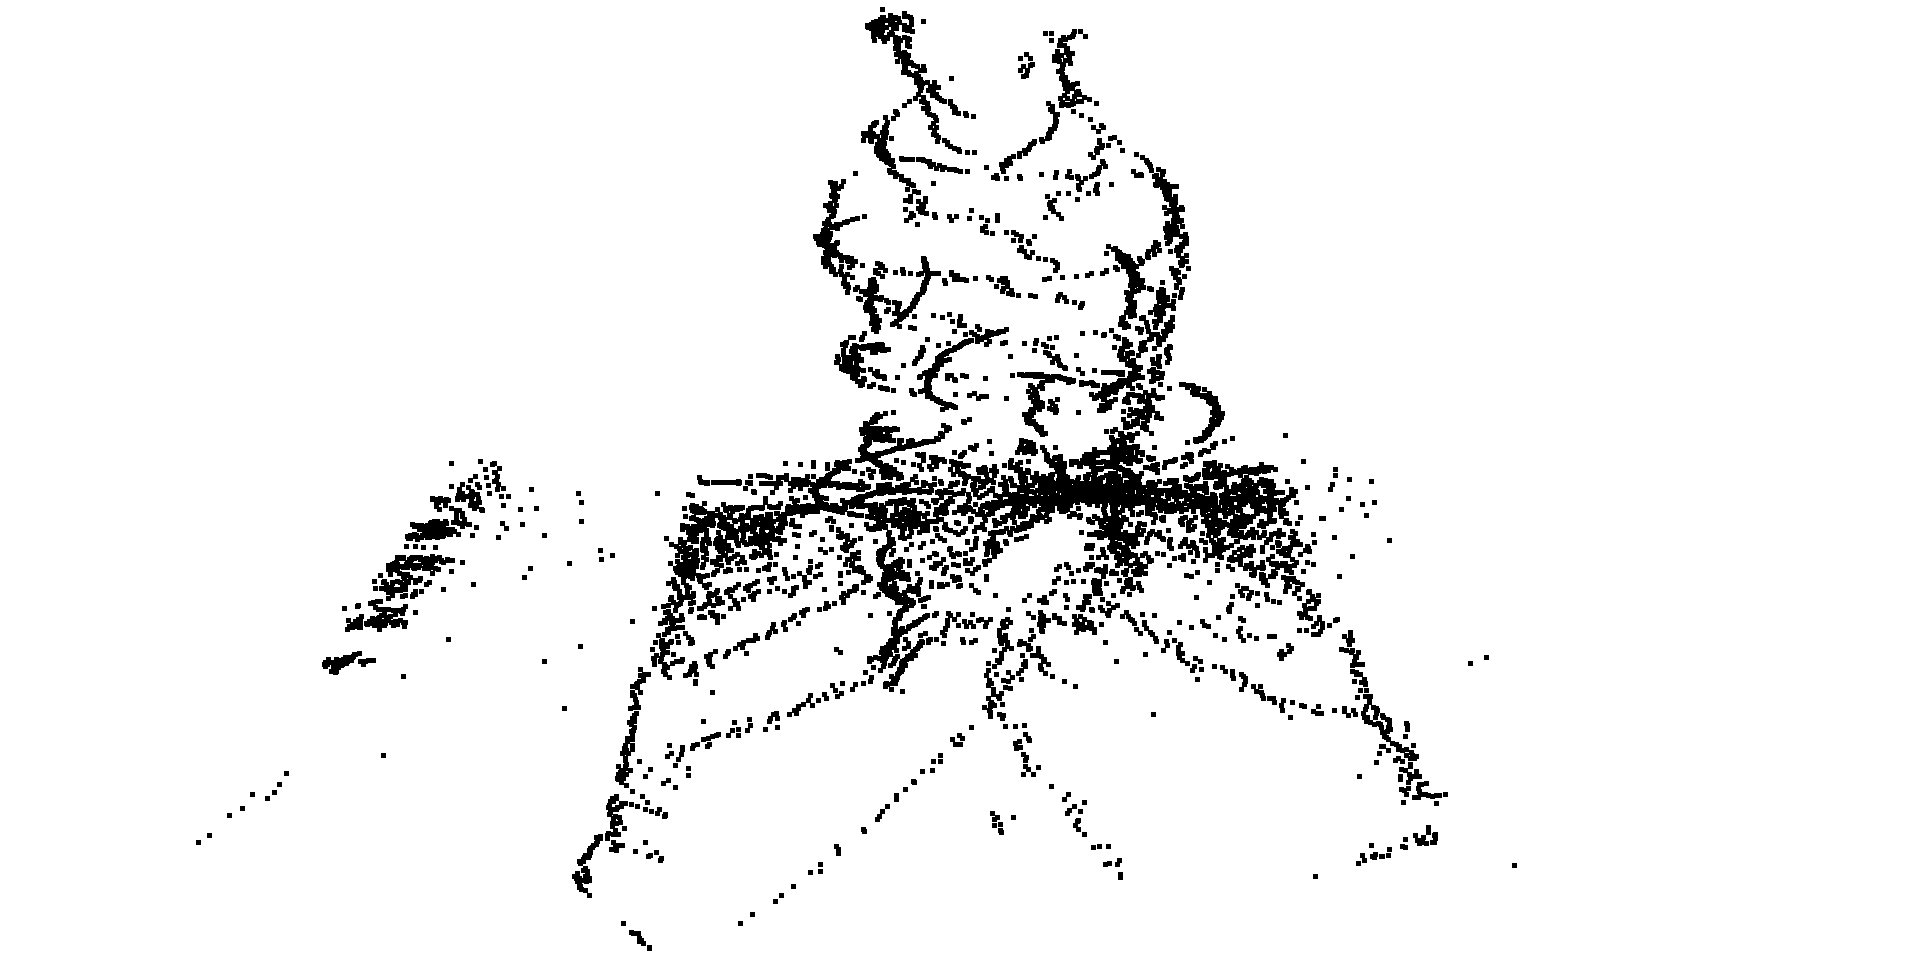
\includegraphics[width=.45\linewidth]{img/stay.png}
    \label{pcstay}
  }
  \subfloat[Typing]{
    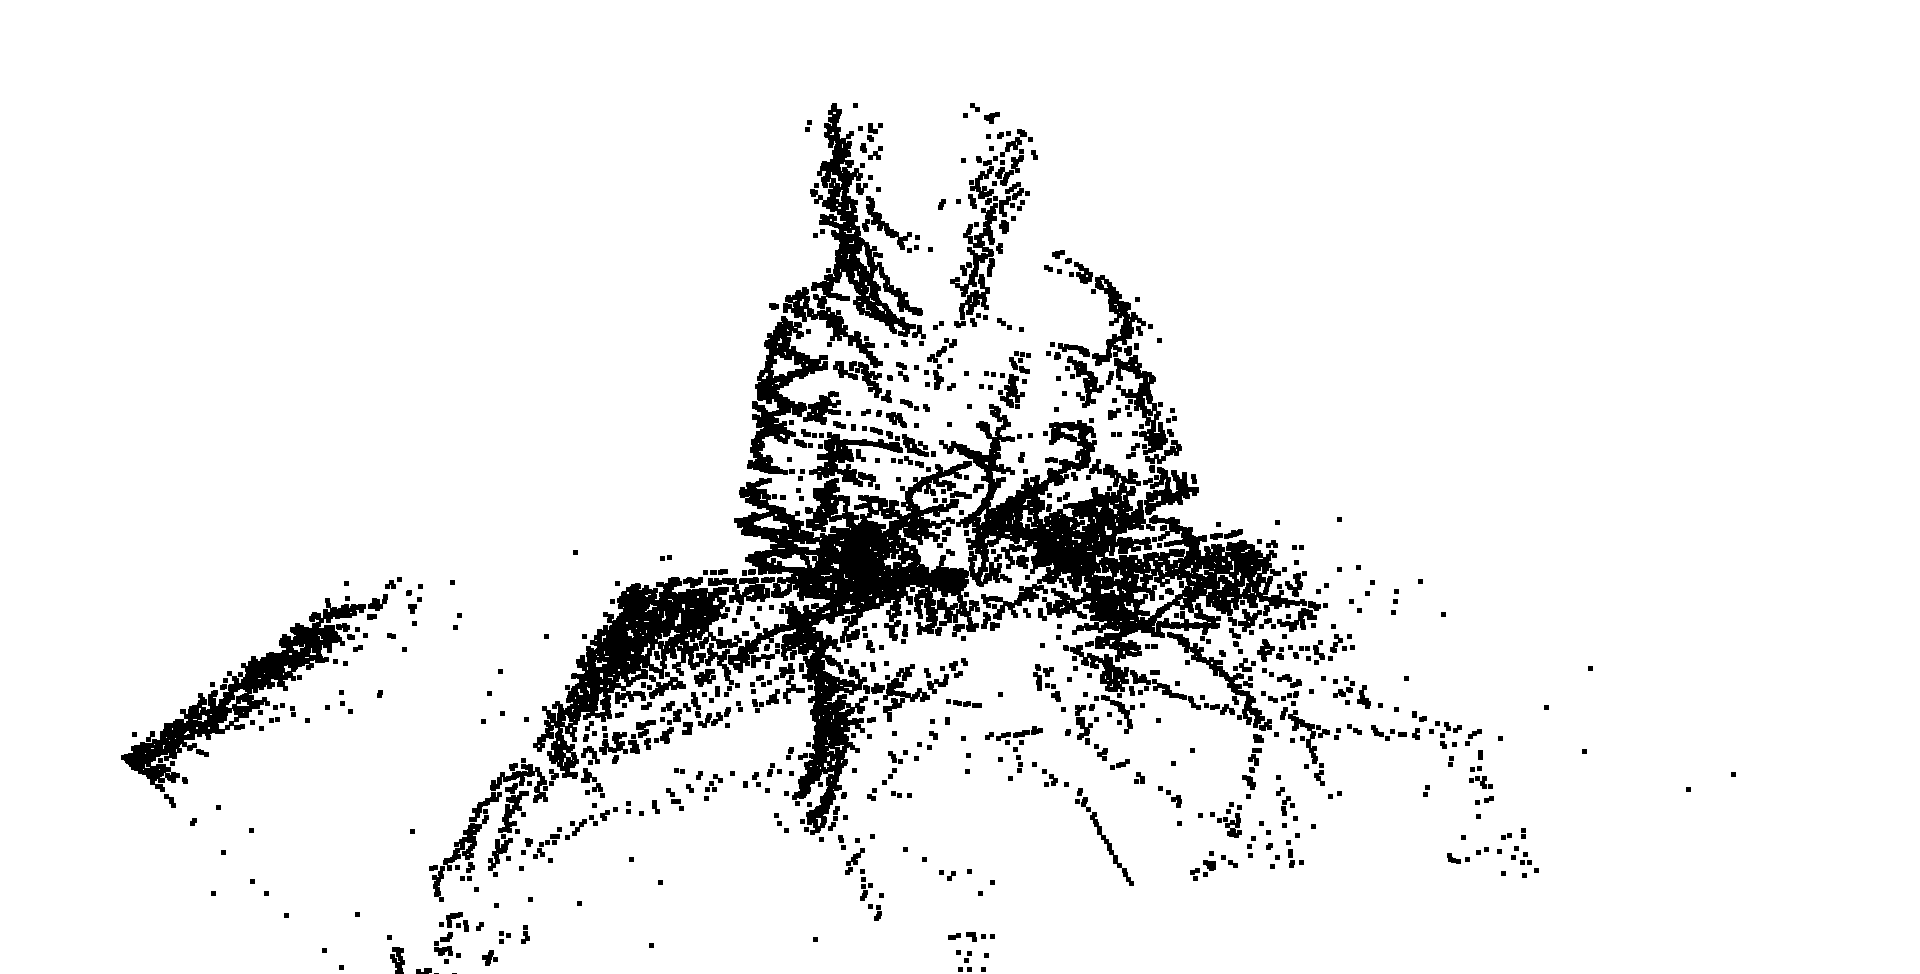
\includegraphics[width=.45\linewidth]{img/typing.png}
    \label{pctyp}
  }
  \caption{Visualization of data showing each label.}
  \label{labels}
\end{figure} 

\subsection{Processing of proposed system}
%sec:j
%1st paragraph
%1
\revised{Processing followed Section~\ref{sec:method}: two vertices defined each person region for trimming; Open3D extracted normals, dimensionality features, proportion of variance, and FPFH \cite{zhou2018open3d}.}
  %1-1 点座標のみは評価しない
  \revised{We do not evaluate point coordinates only on the basis of the comparison in existing research \cite{DBLP:journals/corr/QiYSG17}.}
    %1-1-1
    \revised{The research evaluated point coordinates only and point coordinates with point features.}
    %1-1-2
    \revised{The research reported higher accuracy with point coordinates and point features than with point coordinates only.}
\begin{deletedblock}
In our experiment, the proposed system was processed according to the methodology described in Section~\ref{sec:method}.
  Two vertices of the region where a person is located were determined and then the point clouds were trimmed. 
The features were generated using the process explained in Section~\ref{sec:method}. 
  Specifically, the normal estimator from Open3D was used and normals were stored with the coordinate data in point cloud data files. 
  The covariances were generated and then the dimensionality features and the proportion of variance were calculated. 
  The FPFH estimator from Open3D was utilized and the FPFH values were stored in a separate file from the coordinate data. 
\end{deletedblock}
  %1-2
  \revised{DBSCAN and k-means removed outliers as in Section~\ref{sec:method}; point counts were adjusted to 4,096 after clustering and downsampling \cite{pytorchpointnet++}.}
  \begin{deletedblock}
  The data were clustered using the process explained in Section~\ref{sec:method}. 
    Specifically, outliers and some clusters were removed after implementing DBSCAN.
    Some clusters were also removed after performing k-means. 
  After the clustering and downsampling, the number of points in each point cloud was adjusted to 4,096, which is the default value of the Github repository \cite{pytorchpointnet++}. 
  \end{deletedblock}
  %1-3
  Normalization was performed using different values for each point cloud dataset used for the training. 
  %1-4
  \deleted{PointCutMix augmented normalized training data by replacing the top $\lambda$\% of nearest-neighbor-matched points between three point clouds A, B, and C, with $\lambda$ drawn from a beta distribution \cite{ZHANG202258}.}
  \revised{PointCutMix augmented normalized training data by replacing the top $\lambda$\% of nearest-neighbor-matched points among three point clouds, with $\lambda$ drawn from a beta distribution \cite{ZHANG202258}.}
  %1-4-1
  \deleted{PointCutMix increases shape diversity among training samples and improves robustness to subject-dependent point-cloud density.}
  \revised{PointCutMix increases shape diversity among training samples and improves robustness to experiment-participant-dependent point cloud density.}
  \begin{deletedblock}
  Data augmentation was performed on the normalized data. 
    For data augmentation, PointCutmix was used\cite{ZHANG202258}. 
        Three point clouds A, B, and C were prepared. 
        The beta function was used to randomly determine a real number $\lambda$. 
        Points from point cloud B were assigned to each point in point cloud A. 
            For each point in A, the distance to all points in B was measured and the index of the closest point in B was assigned. 
            Then, the top $\lambda$\% of points in A, sorted by distance, were replaced with their assigned points from B. 
        Points from point cloud C were assigned to each point in point cloud A. 
            For each point in A, the distance to all points in B was measured and the index of the closest point in C was assigned. 
            Then, the top $\lambda$\% of points in A, sorted by distance, were replaced with their assigned points from C. 
  \end{deletedblock}

%2nd paragraph
%2
\deleted{Data were split 4:1 for training and validation; multi-scale grouping (MSG) formed PointNet++ groups \cite{pytorchpointnet++,PytorchPointnetPointnet2}.}
\begin{revisedblock}
We split frames of each of the three experiment participants at a ratio of 4:1.
  %2-1
  Four fifths of the frames were used for training.
  %2-2
  One fifth of the frames were used for validation.
%3
Multi-scale grouping (MSG) formed PointNet++ groups \cite{pytorchpointnet++,PytorchPointnetPointnet2}.
\end{revisedblock}
\begin{deletedblock}
The remaining data were split into 4:1 for the training and validation. 
Multi-scale grouping (MSG) was used to create groups in PointNet++, as based on prior methods \cite{pytorchpointnet++,PytorchPointnetPointnet2}.
An output containing the parameters of the classification was created after the training was completed. 
\end{deletedblock}


\subsection{Evaluation metric}
% \begin{spverbatim}
%1
% We evaluated the classification models trained using the data from one subject and the test data from one of the other subjects. 
%   %1-1
%   For example, we evaluated the classification model for A data using the B or C test data. 
%   %1-2
%   As shown in the Table~\ref{pattern}, there are six different evaluation patterns for the combination of one person's classification model and another person's test data. 

%1評価方法
\deleted{We evaluated the classification models trained using the augmented data from three subjects and the test data from nine subjects.}
\revised{The classification models trained using the augmented data from three subjects were evaluated using the test data from twenty-eight subjects.} 

%2精度計算
Accuracy was utilized to evaluate the classification models, defined as
  %2-1s
  % We defined accuracy used in the evaluation as follows:
  \begin{equation}
    \begin{split}
      \frac{TM+TP+TS+TT}{TM+TP+TS+TT+FM+FP+FS+FT}, 
    \end{split}
  \end{equation}
where $TM$ is the number of correctly classified point clouds that actually indicate the mouse operation, $TP$, $TS$, and $TT$ are the number of correctly classified point clouds that actually indicate the pad operation, the sitting still without moving, and the typing, respectively, and $FM$, $FP$, $FS$, and $FT$ are the number of point clouds that were not correctly classified. 
% \end{spverbatim}

% \begin{table}[b]
%   \centering
% 	\caption{Combination of training and test data for evaluation.}
% 	\label{pattern}
% 	\begin{tabular}{c|c|c|}
%     \hline
%     & \textbf{Training} & \textbf{Test}\\ \hline
%     1 & A & B\\
%     2 & A & C\\
%     3 & B & A\\
%     4 & B & C\\
%     5 & C & A\\
%     6 & C & B\\
%     \hline
%  \end{tabular}
% \end{table}
            
\section{Evaluation}
\label{sec:evaluation}
\subsection{Validation results}
%6/27 tb ⇒ t
\begin{figure}[t]
    \centering
    \subfloat[Normals]{
      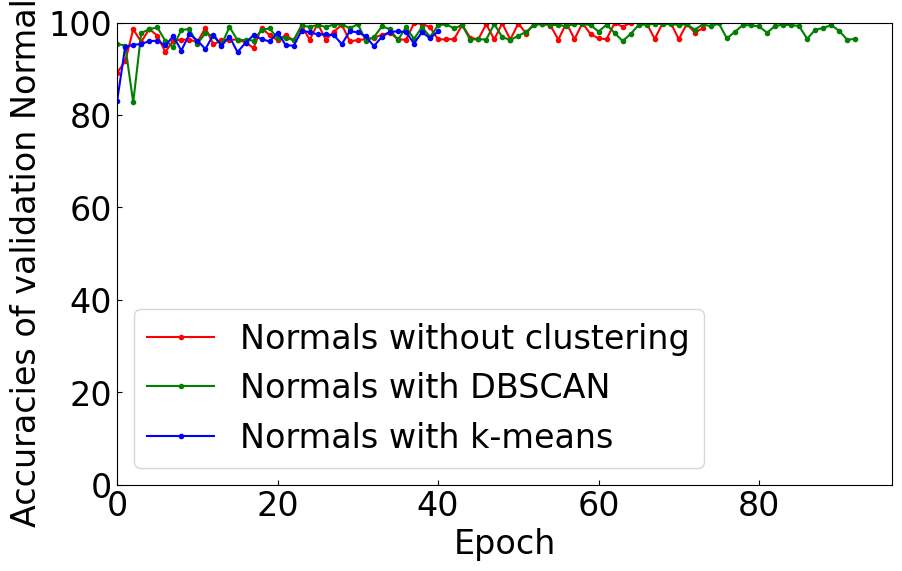
\includegraphics[width=.45\linewidth]{img/Accuracies_of_validation_normals.png}
      \label{valnormal}
    }
    \subfloat[Dimensionality features]{
      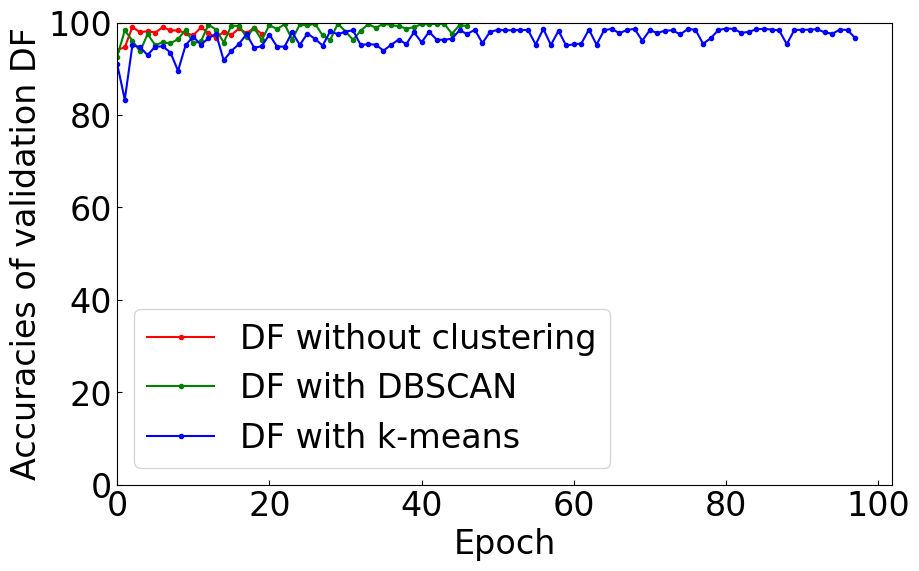
\includegraphics[width=.45\linewidth]{img/Accuracies_of_validation_DF.png}
      \label{valdim}
    }
    \\
    \subfloat[Proportion of variances]{
      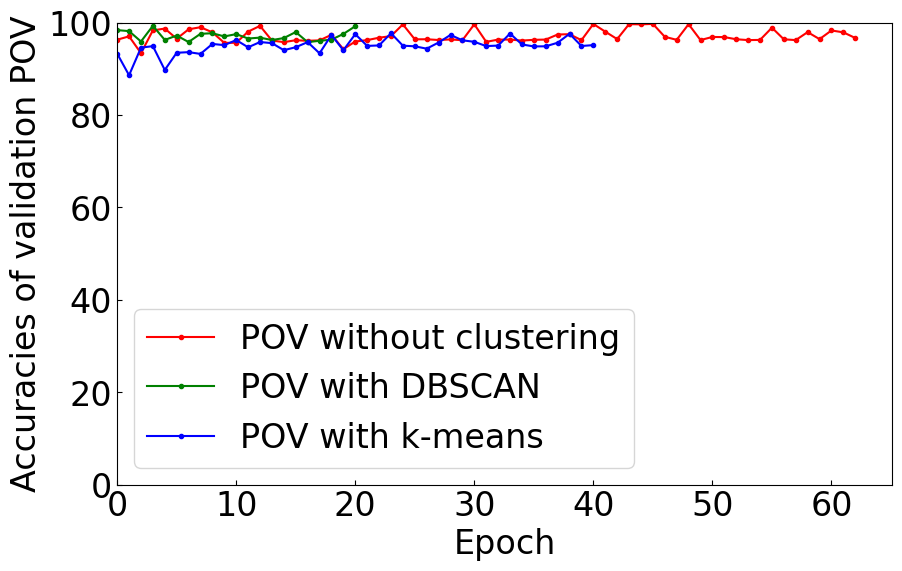
\includegraphics[width=.45\linewidth]{img/Accuracies_of_validation_POV.png}
      \label{valproportion}
    }
    \subfloat[FPFH]{
      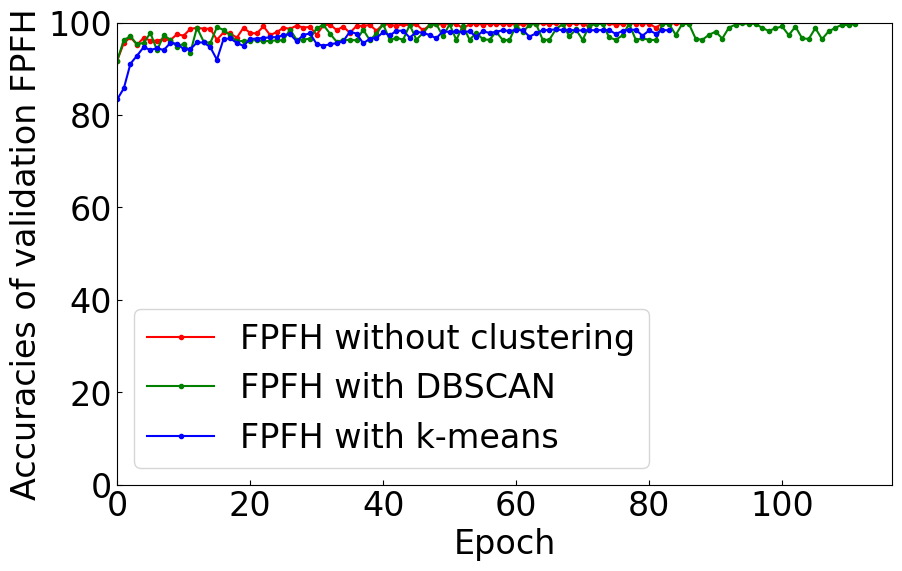
\includegraphics[width=.45\linewidth]{img/Accuracies_of_validation_FPFH.png}
      \label{valfpfh}
    }
    \caption{Classification accuracies of validation.}
    \label{valacc}
  \end{figure} 

%1st paragraph
%1概要
\deleted{Fig.~\ref{valacc} show graphs of the validation per epoch when using each feature.}
\deleted{%2各表の折れ線グラフの説明
Each figure has three line graphs, each with no clustering, with DBSCAN, and with k-means.}
\revised{Fig.~\ref{valacc} plots validation accuracy per epoch for each feature with no clustering, DBSCAN, and k-means.}
\begin{deletedblock}
%2nd paragraph
%1法線を使った分類モデル
Fig.~\ref{valacc}\subref{valnormal} shows the accuracies of three types classification models when the normals were used. 
    %1-1
    As shown, the overall accuracies are nearly 100\%. 
%2The dimensionality featuresを使った分類モデル
Fig.~\ref{valacc}\subref{valdim} shows the accuracies of three types classification models when the dimensionality features were used. 
    %2-1
    As shown, the overall accuracies are nearly 100\%. 
%3The proportion of varianceを使った分類モデル
Fig.~\ref{valacc}\subref{valproportion} shows the accuracies of three types classification models when the proportion of variance was used. 
  %3-1
  As shown, the overall accuracies are nearly 100\%. 
%4FPFHの分類モデル
Fig.~\ref{valacc}\subref{valfpfh} shows the accuracies of three types classification models when the FPFH was used. 
  %4-1
  As shown, the overall accuracies are nearly 100\%. 
\end{deletedblock}
%2
\revised{All four features achieved nearly 100\% validation accuracy across clustering methods.}

%2nd paragraph
%5エポック数の決定
\deleted{The training epochs for each classification model were set so that after updating the best accuracy in validation, training would be terminated if there were no updates within 15 epochs.}
\revised{Training was terminated after 15 epochs without validation-accuracy improvement beyond the best value.}


\subsection{Accuracy}
%1st paragraph
%1
Table~\ref{accresults} shows the accuracy for all twelve combinations of features and clustering methods used.
%2
\deleted{Subjects A to AB served as the test dataset for four posture classes.}
\revised{Experiment participants A to AB served as the test dataset for four posture classes.}
\revised{Four posture classes yield a 25\% baseline accuracy under uniform random guessing.}
\revised{Accuracy exceeded the 25\% baseline in all cases in Table~\ref{accresults}.}
%3
\deleted{Depending on the feature and clustering combination, test accuracy was stable or varied across test subjects in Table~\ref{accresults}.}
\revised{Depending on the feature and clustering combination, test accuracy was stable or varied across test experiment participants in Table~\ref{accresults}.}
\deleted{Classification accuracy varied across test subjects because point-cloud density and body size differed from the three training subjects.}
\begin{deletedblock}
The accuracy is reported with the data from subjects A to AB serving as the test dataset.
Since we are classifying 4 posture classes, a baseline accuracy of 25\% or higher is expected. 
In all cases Table~\ref{accresults}, the accuracy exceeded the baseline.
\end{deletedblock}

%2nd paragraph
%4
Regarding the clustering methods, no clustering or DBSCAN tended to achieve higher accuracy than K-means.
  %4-1
  \revised{k-means tended to achieve lower accuracy than no clustering or DBSCAN for the same feature type.}
  \deleted{k-means tended to lower accuracy by removing hand-region points required to distinguish typing from pad operation.}

%3rd paragraph
%5
In terms of features, normals tended to yield higher accuracy when no clustering or DBSCAN was employed.
  %5-1
  \revised{Classification using normals yielded comparatively stable test accuracy in Table~\ref{accresults}.}
  \deleted{Normals yielded stable test accuracy when no clustering or DBSCAN was applied.}
  %5-2
  \deleted{Dimensionality features resulted in higher accuracies than the other three feature types for several test subjects outside the training set of subjects A, B, and C in Table~\ref{accresults}.}
  \revised{Dimensionality features resulted in higher accuracies than the other three feature types for several test experiment participants outside the training set of experiment participants A, B, and C in Table~\ref{accresults}.}
  \deleted{Dimensionality features achieved higher accuracy than other features for several subjects outside the training set when local shape resembled training examples.}

\begin{table*}[b]
  \centering
  \caption{Classification accuracy for each subject and feature and clustering combination.}
  \label{accresults}
  \footnotesize
  \setlength{\tabcolsep}{3pt}
  \resizebox{\textwidth}{!}{%
  \begin{tabular}{@{}c*{12}{c}@{}}
    \toprule
    & \multicolumn{3}{c}{Normals} & \multicolumn{3}{c}{Dim.\ features} & \multicolumn{3}{c}{Prop.\ variance} & \multicolumn{3}{c}{FPFH} \\
    \cmidrule(lr){2-4}\cmidrule(lr){5-7}\cmidrule(lr){8-10}\cmidrule(lr){11-13}
    Subject &
    \multicolumn{1}{c}{\label{normalnone}None} & \multicolumn{1}{c}{\label{normaldbscan}DBSCAN} & \multicolumn{1}{c}{\label{normalkmeans}k-means} &
    \multicolumn{1}{c}{\label{dimnone}None} & \multicolumn{1}{c}{\label{dimdbscan}DBSCAN} & \multicolumn{1}{c}{\label{dimkmeans}k-means} &
    \multicolumn{1}{c}{\label{proportionnone}None} & \multicolumn{1}{c}{\label{proportiondbscan}DBSCAN} & \multicolumn{1}{c}{\label{proportionkmeans}k-means} &
    \multicolumn{1}{c}{\label{fpfhnone}None} & \multicolumn{1}{c}{\label{fpfhdbscan}DBSCAN} & \multicolumn{1}{c}{\label{fpfhkmeans}k-means} \\
    \midrule
A & $0.65$ & $0.71$ & $0.60$ & $0.43$ & $0.86$ & $0.79$ & $0.70$ & $0.82$ & $0.70$ & $0.73$ & $0.85$ & $0.75$ \\
B & $0.98$ & $0.99$ & $0.88$ & $0.94$ & $0.97$ & $0.92$ & $0.98$ & $0.91$ & $0.82$ & $0.99$ & $0.96$ & $0.89$ \\
C & $0.70$ & $0.70$ & $0.70$ & $0.70$ & $0.70$ & $0.70$ & $0.70$ & $0.70$ & $0.70$ & $0.70$ & $0.70$ & $0.70$ \\
D & $0.61$ & $0.72$ & $0.41$ & $0.59$ & $0.67$ & $0.63$ & $0.47$ & $0.44$ & $0.63$ & $0.50$ & $0.60$ & $0.55$ \\
E & $0.63$ & $0.69$ & $0.46$ & $0.73$ & $0.60$ & $0.59$ & $0.60$ & $0.58$ & $0.56$ & $0.66$ & $0.53$ & $0.57$ \\
F & $0.72$ & $0.75$ & $0.54$ & $0.83$ & $0.58$ & $0.56$ & $0.61$ & $0.55$ & $0.62$ & $0.76$ & $0.58$ & $0.50$ \\
G & $0.68$ & $0.75$ & $0.40$ & $0.72$ & $0.53$ & $0.54$ & $0.56$ & $0.55$ & $0.54$ & $0.75$ & $0.55$ & $0.40$ \\
H & $0.71$ & $0.74$ & $0.68$ & $0.75$ & $0.68$ & $0.66$ & $0.60$ & $0.62$ & $0.61$ & $0.72$ & $0.63$ & $0.69$ \\
I & $0.76$ & $0.90$ & $0.63$ & $0.92$ & $0.66$ & $0.65$ & $0.61$ & $0.61$ & $0.60$ & $0.75$ & $0.64$ & $0.62$ \\
J & $0.72$ & $0.89$ & $0.88$ & $0.68$ & $0.90$ & $0.75$ & $0.73$ & $0.80$ & $0.84$ & $0.95$ & $0.81$ & $0.92$ \\
K & $0.74$ & $0.87$ & $0.87$ & $0.97$ & $0.86$ & $0.77$ & $0.65$ & $0.82$ & $0.79$ & $0.83$ & $0.80$ & $0.80$ \\
L & $0.73$ & $0.83$ & $0.90$ & $1.00$ & $0.86$ & $0.81$ & $0.63$ & $0.83$ & $0.80$ & $0.80$ & $0.81$ & $0.85$ \\
M & $0.59$ & $0.59$ & $0.45$ & $0.56$ & $0.60$ & $0.44$ & $0.56$ & $0.46$ & $0.40$ & $0.49$ & $0.60$ & $0.45$ \\
N & $0.67$ & $0.60$ & $0.62$ & $0.63$ & $0.76$ & $0.75$ & $0.84$ & $0.60$ & $0.68$ & $0.75$ & $0.84$ & $0.68$ \\
O & $0.85$ & $0.71$ & $0.71$ & $0.70$ & $0.76$ & $0.73$ & $0.73$ & $0.61$ & $0.68$ & $0.80$ & $0.73$ & $0.72$ \\
P & $0.79$ & $0.72$ & $0.70$ & $0.70$ & $0.82$ & $0.77$ & $0.68$ & $0.56$ & $0.75$ & $0.81$ & $0.80$ & $0.76$ \\
Q & $0.70$ & $0.67$ & $0.68$ & $0.70$ & $0.70$ & $0.64$ & $0.66$ & $0.60$ & $0.64$ & $0.71$ & $0.70$ & $0.68$ \\
R & $0.90$ & $0.88$ & $0.92$ & $0.72$ & $0.99$ & $0.84$ & $0.84$ & $0.89$ & $0.78$ & $0.80$ & $1.00$ & $0.87$ \\
S & $0.68$ & $0.72$ & $0.78$ & $0.92$ & $0.80$ & $0.73$ & $0.60$ & $0.79$ & $0.65$ & $0.59$ & $0.71$ & $0.83$ \\
T & $0.93$ & $0.87$ & $0.70$ & $0.70$ & $0.79$ & $0.67$ & $0.79$ & $0.70$ & $0.71$ & $0.85$ & $0.91$ & $0.74$ \\
U & $0.69$ & $0.81$ & $0.85$ & $0.71$ & $0.91$ & $0.76$ & $0.80$ & $0.89$ & $0.82$ & $0.87$ & $0.80$ & $0.86$ \\
V & $0.62$ & $0.62$ & $0.82$ & $0.74$ & $0.64$ & $0.66$ & $0.61$ & $0.57$ & $0.70$ & $0.54$ & $0.57$ & $0.66$ \\
W & $0.62$ & $0.63$ & $0.65$ & $0.32$ & $0.58$ & $0.56$ & $0.56$ & $0.57$ & $0.50$ & $0.41$ & $0.62$ & $0.41$ \\
X & $0.61$ & $0.65$ & $0.47$ & $0.36$ & $0.64$ & $0.48$ & $0.53$ & $0.60$ & $0.47$ & $0.41$ & $0.57$ & $0.43$ \\
Y & $0.60$ & $0.59$ & $0.64$ & $0.61$ & $0.67$ & $0.62$ & $0.60$ & $0.63$ & $0.60$ & $0.60$ & $0.65$ & $0.61$ \\
Z & $0.62$ & $0.59$ & $0.68$ & $0.77$ & $0.68$ & $0.58$ & $0.60$ & $0.64$ & $0.55$ & $0.66$ & $0.67$ & $0.66$ \\
AA & $0.64$ & $0.87$ & $0.94$ & $0.90$ & $0.79$ & $0.88$ & $0.62$ & $0.76$ & $0.71$ & $0.58$ & $0.54$ & $0.63$ \\
AB & $0.70$ & $0.90$ & $0.96$ & $0.82$ & $0.94$ & $0.87$ & $0.68$ & $0.94$ & $0.83$ & $0.87$ & $0.72$ & $0.86$ \\
    \bottomrule
  \end{tabular}%
  }
\end{table*}

%4th paragraph (C.2-1; after C.1-6 three-class paragraph when present)
\begin{revisedblock}
%6
We report four-class and three-class confusion counts on test data A.
%7
For normals without clustering, pad operation yielded 172 false predictions as mouse operation.
  %7-1
  Typing yielded 103 false predictions as pad operation.
%8
For normals with DBSCAN, pad operation yielded 30 false predictions as mouse operation.
  %8-1
  Typing yielded 230 false predictions as pad operation.
%9
For normals without clustering, pad-or-typing yielded 189 false predictions as mouse operation.
%10
For normals with DBSCAN, pad-or-typing yielded 30 false predictions as mouse operation.
%11
Full four-class and three-class confusion matrices for all twelve preprocessing configurations appear in the response letter.
\end{revisedblock}


% \subsection{Confusion matrices}
% %分類モデルごとの各表の説明
%|-テストデータごとの表の説明
% |-表から読み取れること
% |-考察

% \noindent{\red{Todo:左LiDARの6組について、テストデータからStayをなしにした3分類での精度表とマトリクスを示し、精度が上がる/下がるかを考察する。}}\\

% NOTE:
% - Tables are generated into tex/evaluation/confusion-matrices/table.tex

% Confusion matrices (text only; tables are in confusion-matrices-tables.tex)

Tables~\ref{normalnonematrix} and \ref{normalkmeansmatrix} present \deleted{confusion matrices for each subject} \revised{representative confusion matrices for test subjects A to AB}.
%
The rows represent the ground truth labels, and the columns represent the inferred labels.
%
\deleted{Table~\ref{normalnonematrix} and Table~\ref{normalkmeansmatrix} correspond to the results shown in Table~\ref{accresults}(a) and Table~\ref{accresults}(i), respectively.}
%
\begin{revisedblock}
We compare two conditions to examine the effect of clustering.
  %
  The conditions are: normals without clustering and normals with k-means.
\end{revisedblock}
%
\deleted{Both of these used normals as features; however, Table~\ref{accresults}(a) exhibited high accuracy, while Table~\ref{accresults}(i) showed lower accuracy.}
\revised{Both of the used normals as features; however, the normals without clustering tended to show higher accuracy, while the normals with k-means tended to show lower accuracy in Table~\ref{accresults}.}
%
In Table~\ref{normalnonematrix}, the diagonal elements from the top-left to the bottom-right are large, indicating that the inferred labels largely agreed with the ground truth. 
%
However, there were frequent misclassifications of typing as pad operation. 
%
This is likely due to the difficulty in distinguishing whether both hands were touching the pad or the keyboard. 
%
In Table~\ref{normalkmeansmatrix}, in addition to misclassifying typing as pad operation, there were also frequent misclassifications of pad operation as typing.
  
  
% NOTE: subfig's default (a)...(z) overflows for 28 subfloats in a table
% (uses the `subtable` counter). Use numeric labels locally.
{
\renewcommand{\thesubtable}{\arabic{subtable}}
% Auto-generated confusion matrices for subjects A--AB (representative conditions)
% Regenerate: powershell -ExecutionPolicy Bypass -File tex/evaluation/generate_confusion_matrices_A_AB.ps1

\begin{table}[b]
  \centering
  \caption{Matrix of test results with normals and without clustering method. Diagonal toward lower right corner is correct. Vertical columns represent number of labels inferred as mouse operation, pad operation, sitting still, and typing, respectively, from left to right. Horizontal rows represent, from top, number of labels where actual label is mouse operation, pad operation, sitting still, or typing.}
  \label{normalnonematrix}
  \subfloat[Test data A]{
    \label{nnA}
    \scalebox{0.67}{
      \begin{tabular}{|c|c|c|c|}
      \hline
        $273$ & $0$ & $0$ & $0$ \\ \cline{1-4}
        $172$ & $99$ & $2$ & $1$ \\ \cline{1-4}
        $1$ & $0$ & $95$ & $0$ \\ \cline{1-4}
        $17$ & $103$ & $25$ & $131$ \\ \cline{1-4}
      \hline
    \end{tabular}
    }
  }
  \hfill
  \subfloat[Test data B]{
    \label{nnB}
    \scalebox{0.67}{
      \begin{tabular}{|c|c|c|c|}
      \hline
        $272$ & $3$ & $2$ & $0$ \\ \cline{1-4}
        $0$ & $265$ & $3$ & $7$ \\ \cline{1-4}
        $0$ & $1$ & $92$ & $0$ \\ \cline{1-4}
        $0$ & $2$ & $0$ & $274$ \\ \cline{1-4}
      \hline
    \end{tabular}
    }
  }
  \hfill
  \subfloat[Test data C]{
    \label{nnC}
    \scalebox{0.67}{
      \begin{tabular}{|c|c|c|c|}
      \hline
        $279$ & $0$ & $0$ & $0$ \\ \cline{1-4}
        $0$ & $0$ & $0$ & $278$ \\ \cline{1-4}
        $0$ & $0$ & $94$ & $0$ \\ \cline{1-4}
        $0$ & $0$ & $0$ & $276$ \\ \cline{1-4}
      \hline
    \end{tabular}
    }
  }
  \hfill
  \subfloat[Test data D]{
    \label{nnD}
    \scalebox{0.67}{
      \begin{tabular}{|c|c|c|c|}
      \hline
        $267$ & $9$ & $1$ & $0$ \\ \cline{1-4}
        $48$ & $185$ & $43$ & $3$ \\ \cline{1-4}
        $0$ & $6$ & $89$ & $0$ \\ \cline{1-4}
        $0$ & $252$ & $1$ & $22$ \\ \cline{1-4}
      \hline
    \end{tabular}
    }
  }
  \hfill
  \subfloat[Test data E]{
    \label{nnE}
    \scalebox{0.67}{
      \begin{tabular}{|c|c|c|c|}
      \hline
        $275$ & $1$ & $0$ & $2$ \\ \cline{1-4}
        $0$ & $275$ & $2$ & $0$ \\ \cline{1-4}
        $0$ & $63$ & $34$ & $0$ \\ \cline{1-4}
        $0$ & $272$ & $1$ & $4$ \\ \cline{1-4}
      \hline
    \end{tabular}
    }
  }
  \hfill
  \subfloat[Test data F]{
    \label{nnF}
    \scalebox{0.67}{
      \begin{tabular}{|c|c|c|c|}
      \hline
        $276$ & $2$ & $2$ & $0$ \\ \cline{1-4}
        $0$ & $270$ & $5$ & $4$ \\ \cline{1-4}
        $2$ & $4$ & $90$ & $1$ \\ \cline{1-4}
        $0$ & $241$ & $0$ & $38$ \\ \cline{1-4}
      \hline
    \end{tabular}
    }
  }
  \hfill
  \subfloat[Test data G]{
    \label{nnG}
    \scalebox{0.67}{
      \begin{tabular}{|c|c|c|c|}
      \hline
        $270$ & $7$ & $2$ & $0$ \\ \cline{1-4}
        $0$ & $280$ & $0$ & $0$ \\ \cline{1-4}
        $0$ & $39$ & $56$ & $0$ \\ \cline{1-4}
        $0$ & $255$ & $0$ & $24$ \\ \cline{1-4}
      \hline
    \end{tabular}
    }
  }
  \hfill
  \subfloat[Test data H]{
    \label{nnH}
    \scalebox{0.67}{
      \begin{tabular}{|c|c|c|c|}
      \hline
        $279$ & $0$ & $0$ & $0$ \\ \cline{1-4}
        $0$ & $274$ & $1$ & $2$ \\ \cline{1-4}
        $1$ & $15$ & $79$ & $0$ \\ \cline{1-4}
        $0$ & $254$ & $0$ & $25$ \\ \cline{1-4}
      \hline
    \end{tabular}
    }
  }
  \hfill
  \subfloat[Test data I]{
    \label{nnI}
    \scalebox{0.67}{
      \begin{tabular}{|c|c|c|c|}
      \hline
        $279$ & $0$ & $0$ & $0$ \\ \cline{1-4}
        $0$ & $274$ & $3$ & $2$ \\ \cline{1-4}
        $0$ & $42$ & $55$ & $0$ \\ \cline{1-4}
        $0$ & $179$ & $0$ & $100$ \\ \cline{1-4}
      \hline
    \end{tabular}
    }
  }
  \hfill
  \subfloat[Test data J]{
    \label{nnJ}
    \scalebox{0.67}{
      \begin{tabular}{|c|c|c|c|}
      \hline
        $264$ & $0$ & $0$ & $0$ \\ \cline{1-4}
        $0$ & $266$ & $0$ & $0$ \\ \cline{1-4}
        $0$ & $9$ & $73$ & $0$ \\ \cline{1-4}
        $81$ & $153$ & $0$ & $30$ \\ \cline{1-4}
      \hline
    \end{tabular}
    }
  }
  \hfill
  \subfloat[Test data K]{
    \label{nnK}
    \scalebox{0.67}{
      \begin{tabular}{|c|c|c|c|}
      \hline
        $268$ & $0$ & $0$ & $0$ \\ \cline{1-4}
        $0$ & $265$ & $0$ & $1$ \\ \cline{1-4}
        $0$ & $9$ & $75$ & $0$ \\ \cline{1-4}
        $0$ & $218$ & $0$ & $49$ \\ \cline{1-4}
      \hline
    \end{tabular}
    }
  }
  \hfill
  \subfloat[Test data L]{
    \label{nnL}
    \scalebox{0.67}{
      \begin{tabular}{|c|c|c|c|}
      \hline
        $267$ & $0$ & $0$ & $0$ \\ \cline{1-4}
        $0$ & $267$ & $0$ & $0$ \\ \cline{1-4}
        $0$ & $3$ & $81$ & $0$ \\ \cline{1-4}
        $0$ & $240$ & $0$ & $26$ \\ \cline{1-4}
      \hline
    \end{tabular}
    }
  }
  \hfill
  \subfloat[Test data M]{
    \label{nnM}
    \scalebox{0.67}{
      \begin{tabular}{|c|c|c|c|}
      \hline
        $257$ & $0$ & $1$ & $9$ \\ \cline{1-4}
        $0$ & $0$ & $0$ & $267$ \\ \cline{1-4}
        $0$ & $0$ & $0$ & $86$ \\ \cline{1-4}
        $0$ & $0$ & $0$ & $265$ \\ \cline{1-4}
      \hline
    \end{tabular}
    }
  }
  \hfill
  \subfloat[Test data N]{
    \label{nnN}
    \scalebox{0.67}{
      \begin{tabular}{|c|c|c|c|}
      \hline
        $265$ & $0$ & $0$ & $0$ \\ \cline{1-4}
        $0$ & $62$ & $0$ & $206$ \\ \cline{1-4}
        $0$ & $0$ & $0$ & $86$ \\ \cline{1-4}
        $0$ & $0$ & $0$ & $267$ \\ \cline{1-4}
      \hline
    \end{tabular}
    }
  }
  \hfill
  \subfloat[Test data O]{
    \label{nnO}
    \scalebox{0.67}{
      \begin{tabular}{|c|c|c|c|}
      \hline
        $267$ & $0$ & $0$ & $0$ \\ \cline{1-4}
        $0$ & $135$ & $0$ & $131$ \\ \cline{1-4}
        $0$ & $0$ & $85$ & $0$ \\ \cline{1-4}
        $0$ & $0$ & $0$ & $265$ \\ \cline{1-4}
      \hline
    \end{tabular}
    }
  }
  \hfill
  \subfloat[Test data P]{
    \label{nnP}
    \scalebox{0.67}{
      \begin{tabular}{|c|c|c|c|}
      \hline
        $267$ & $1$ & $0$ & $0$ \\ \cline{1-4}
        $1$ & $205$ & $0$ & $60$ \\ \cline{1-4}
        $0$ & $0$ & $83$ & $0$ \\ \cline{1-4}
        $2$ & $123$ & $0$ & $142$ \\ \cline{1-4}
      \hline
    \end{tabular}
    }
  }
  \hfill
  \subfloat[Test data Q]{
    \label{nnQ}
    \scalebox{0.67}{
      \begin{tabular}{|c|c|c|c|}
      \hline
        $266$ & $0$ & $0$ & $0$ \\ \cline{1-4}
        $0$ & $1$ & $0$ & $265$ \\ \cline{1-4}
        $0$ & $0$ & $86$ & $0$ \\ \cline{1-4}
        $1$ & $2$ & $0$ & $262$ \\ \cline{1-4}
      \hline
    \end{tabular}
    }
  }
  \hfill
  \subfloat[Test data R]{
    \label{nnR}
    \scalebox{0.67}{
      \begin{tabular}{|c|c|c|c|}
      \hline
        $197$ & $44$ & $26$ & $0$ \\ \cline{1-4}
        $0$ & $265$ & $1$ & $0$ \\ \cline{1-4}
        $0$ & $13$ & $72$ & $0$ \\ \cline{1-4}
        $0$ & $0$ & $0$ & $266$ \\ \cline{1-4}
      \hline
    \end{tabular}
    }
  }
  \hfill
  \subfloat[Test data S]{
    \label{nnS}
    \scalebox{0.67}{
      \begin{tabular}{|c|c|c|c|}
      \hline
        $246$ & $13$ & $6$ & $0$ \\ \cline{1-4}
        $0$ & $266$ & $0$ & $0$ \\ \cline{1-4}
        $0$ & $2$ & $83$ & $0$ \\ \cline{1-4}
        $8$ & $255$ & $0$ & $4$ \\ \cline{1-4}
      \hline
    \end{tabular}
    }
  }
  \hfill
  \subfloat[Test data T]{
    \label{nnT}
    \scalebox{0.67}{
      \begin{tabular}{|c|c|c|c|}
      \hline
        $251$ & $16$ & $0$ & $0$ \\ \cline{1-4}
        $0$ & $253$ & $0$ & $14$ \\ \cline{1-4}
        $0$ & $0$ & $85$ & $0$ \\ \cline{1-4}
        $9$ & $25$ & $0$ & $232$ \\ \cline{1-4}
      \hline
    \end{tabular}
    }
  }
  \hfill
  \subfloat[Test data U]{
    \label{nnU}
    \scalebox{0.67}{
      \begin{tabular}{|c|c|c|c|}
      \hline
        $260$ & $5$ & $2$ & $0$ \\ \cline{1-4}
        $0$ & $263$ & $3$ & $0$ \\ \cline{1-4}
        $1$ & $1$ & $82$ & $0$ \\ \cline{1-4}
        $163$ & $95$ & $0$ & $9$ \\ \cline{1-4}
      \hline
    \end{tabular}
    }
  }
  \hfill
  \subfloat[Test data V]{
    \label{nnV}
    \scalebox{0.67}{
      \begin{tabular}{|c|c|c|c|}
      \hline
        $266$ & $0$ & $0$ & $0$ \\ \cline{1-4}
        $1$ & $241$ & $26$ & $0$ \\ \cline{1-4}
        $0$ & $47$ & $37$ & $0$ \\ \cline{1-4}
        $2$ & $262$ & $1$ & $1$ \\ \cline{1-4}
      \hline
    \end{tabular}
    }
  }
  \hfill
  \subfloat[Test data W]{
    \label{nnW}
    \scalebox{0.67}{
      \begin{tabular}{|c|c|c|c|}
      \hline
        $231$ & $11$ & $24$ & $0$ \\ \cline{1-4}
        $0$ & $245$ & $21$ & $0$ \\ \cline{1-4}
        $0$ & $11$ & $75$ & $0$ \\ \cline{1-4}
        $0$ & $266$ & $0$ & $0$ \\ \cline{1-4}
      \hline
    \end{tabular}
    }
  }
  \hfill
  \subfloat[Test data X]{
    \label{nnX}
    \scalebox{0.67}{
      \begin{tabular}{|c|c|c|c|}
      \hline
        $233$ & $13$ & $21$ & $0$ \\ \cline{1-4}
        $0$ & $225$ & $42$ & $0$ \\ \cline{1-4}
        $0$ & $1$ & $83$ & $0$ \\ \cline{1-4}
        $0$ & $258$ & $9$ & $0$ \\ \cline{1-4}
      \hline
    \end{tabular}
    }
  }
  \hfill
  \subfloat[Test data Y]{
    \label{nnY}
    \scalebox{0.67}{
      \begin{tabular}{|c|c|c|c|}
      \hline
        $267$ & $0$ & $0$ & $0$ \\ \cline{1-4}
        $0$ & $202$ & $65$ & $0$ \\ \cline{1-4}
        $0$ & $19$ & $66$ & $0$ \\ \cline{1-4}
        $8$ & $258$ & $1$ & $0$ \\ \cline{1-4}
      \hline
    \end{tabular}
    }
  }
  \hfill
  \subfloat[Test data Z]{
    \label{nnZ}
    \scalebox{0.67}{
      \begin{tabular}{|c|c|c|c|}
      \hline
        $266$ & $0$ & $0$ & $0$ \\ \cline{1-4}
        $58$ & $198$ & $10$ & $0$ \\ \cline{1-4}
        $0$ & $4$ & $80$ & $0$ \\ \cline{1-4}
        $1$ & $266$ & $0$ & $0$ \\ \cline{1-4}
      \hline
    \end{tabular}
    }
  }
  \hfill
\setcounter{subtable}{0}
  \hfill
  \subfloat[Test data AA]{
    \label{nnAA}
    \scalebox{0.67}{
      \begin{tabular}{|c|c|c|c|}
      \hline
        $253$ & $9$ & $4$ & $0$ \\ \cline{1-4}
        $0$ & $218$ & $49$ & $0$ \\ \cline{1-4}
        $0$ & $4$ & $81$ & $0$ \\ \cline{1-4}
        $3$ & $240$ & $8$ & $14$ \\ \cline{1-4}
      \hline
    \end{tabular}
    }
  }
  \hfill
  \subfloat[Test data AB]{
    \label{nnAB}
    \scalebox{0.67}{
      \begin{tabular}{|c|c|c|c|}
      \hline
        $262$ & $2$ & $2$ & $0$ \\ \cline{1-4}
        $0$ & $263$ & $3$ & $0$ \\ \cline{1-4}
        $0$ & $0$ & $84$ & $0$ \\ \cline{1-4}
        $56$ & $195$ & $3$ & $12$ \\ \cline{1-4}
      \hline
    \end{tabular}
    }
  }
\end{table}

\begin{table}[b]
  \centering
  \caption{Matrix of test results with normals and k-means. Diagonal toward lower right corner is correct. Vertical columns represent number of labels inferred as mouse operation, pad operation, sitting still, and typing, respectively, from left to right. Horizontal rows represent, from top, number of labels where actual label is mouse operation, pad operation, sitting still, or typing.}
  \label{normalkmeansmatrix}
  \subfloat[Test data A]{
    \label{nkA}
    \scalebox{0.67}{
      \begin{tabular}{|c|c|c|c|}
      \hline
        $268$ & $5$ & $0$ & $0$ \\ \cline{1-4}
        $73$ & $197$ & $1$ & $3$ \\ \cline{1-4}
        $7$ & $5$ & $84$ & $0$ \\ \cline{1-4}
        $16$ & $253$ & $3$ & $4$ \\ \cline{1-4}
      \hline
    \end{tabular}
    }
  }
  \hfill
  \subfloat[Test data B]{
    \label{nkB}
    \scalebox{0.67}{
      \begin{tabular}{|c|c|c|c|}
      \hline
        $228$ & $30$ & $12$ & $7$ \\ \cline{1-4}
        $1$ & $254$ & $3$ & $17$ \\ \cline{1-4}
        $12$ & $3$ & $78$ & $0$ \\ \cline{1-4}
        $3$ & $17$ & $1$ & $255$ \\ \cline{1-4}
      \hline
    \end{tabular}
    }
  }
  \hfill
  \subfloat[Test data C]{
    \label{nkC}
    \scalebox{0.67}{
      \begin{tabular}{|c|c|c|c|}
      \hline
        $279$ & $0$ & $0$ & $0$ \\ \cline{1-4}
        $0$ & $0$ & $0$ & $278$ \\ \cline{1-4}
        $0$ & $3$ & $91$ & $0$ \\ \cline{1-4}
        $0$ & $0$ & $0$ & $276$ \\ \cline{1-4}
      \hline
    \end{tabular}
    }
  }
  \hfill
  \subfloat[Test data D]{
    \label{nkD}
    \scalebox{0.67}{
      \begin{tabular}{|c|c|c|c|}
      \hline
        $216$ & $9$ & $17$ & $35$ \\ \cline{1-4}
        $8$ & $57$ & $30$ & $184$ \\ \cline{1-4}
        $9$ & $0$ & $86$ & $0$ \\ \cline{1-4}
        $17$ & $204$ & $29$ & $25$ \\ \cline{1-4}
      \hline
    \end{tabular}
    }
  }
  \hfill
  \subfloat[Test data E]{
    \label{nkE}
    \scalebox{0.67}{
      \begin{tabular}{|c|c|c|c|}
      \hline
        $88$ & $0$ & $0$ & $190$ \\ \cline{1-4}
        $0$ & $273$ & $4$ & $0$ \\ \cline{1-4}
        $0$ & $38$ & $59$ & $0$ \\ \cline{1-4}
        $2$ & $267$ & $4$ & $4$ \\ \cline{1-4}
      \hline
    \end{tabular}
    }
  }
  \hfill
  \subfloat[Test data F]{
    \label{nkF}
    \scalebox{0.67}{
      \begin{tabular}{|c|c|c|c|}
      \hline
        $117$ & $16$ & $147$ & $0$ \\ \cline{1-4}
        $0$ & $263$ & $14$ & $2$ \\ \cline{1-4}
        $0$ & $0$ & $97$ & $0$ \\ \cline{1-4}
        $1$ & $248$ & $4$ & $26$ \\ \cline{1-4}
      \hline
    \end{tabular}
    }
  }
  \hfill
  \subfloat[Test data G]{
    \label{nkG}
    \scalebox{0.67}{
      \begin{tabular}{|c|c|c|c|}
      \hline
        $39$ & $9$ & $231$ & $0$ \\ \cline{1-4}
        $11$ & $232$ & $32$ & $5$ \\ \cline{1-4}
        $0$ & $11$ & $84$ & $0$ \\ \cline{1-4}
        $2$ & $256$ & $2$ & $19$ \\ \cline{1-4}
      \hline
    \end{tabular}
    }
  }
  \hfill
  \subfloat[Test data H]{
    \label{nkH}
    \scalebox{0.67}{
      \begin{tabular}{|c|c|c|c|}
      \hline
        $261$ & $0$ & $0$ & $18$ \\ \cline{1-4}
        $0$ & $271$ & $3$ & $3$ \\ \cline{1-4}
        $0$ & $2$ & $93$ & $0$ \\ \cline{1-4}
        $1$ & $264$ & $6$ & $8$ \\ \cline{1-4}
      \hline
    \end{tabular}
    }
  }
  \hfill
  \subfloat[Test data I]{
    \label{nkI}
    \scalebox{0.67}{
      \begin{tabular}{|c|c|c|c|}
      \hline
        $182$ & $1$ & $95$ & $1$ \\ \cline{1-4}
        $0$ & $275$ & $4$ & $0$ \\ \cline{1-4}
        $1$ & $6$ & $90$ & $0$ \\ \cline{1-4}
        $2$ & $231$ & $9$ & $37$ \\ \cline{1-4}
      \hline
    \end{tabular}
    }
  }
  \hfill
  \subfloat[Test data J]{
    \label{nkJ}
    \scalebox{0.67}{
      \begin{tabular}{|c|c|c|c|}
      \hline
        $264$ & $0$ & $0$ & $0$ \\ \cline{1-4}
        $3$ & $248$ & $0$ & $15$ \\ \cline{1-4}
        $1$ & $62$ & $19$ & $0$ \\ \cline{1-4}
        $8$ & $14$ & $0$ & $242$ \\ \cline{1-4}
      \hline
    \end{tabular}
    }
  }
  \hfill
  \subfloat[Test data K]{
    \label{nkK}
    \scalebox{0.67}{
      \begin{tabular}{|c|c|c|c|}
      \hline
        $253$ & $14$ & $0$ & $1$ \\ \cline{1-4}
        $0$ & $258$ & $2$ & $6$ \\ \cline{1-4}
        $0$ & $84$ & $0$ & $0$ \\ \cline{1-4}
        $0$ & $6$ & $0$ & $261$ \\ \cline{1-4}
      \hline
    \end{tabular}
    }
  }
  \hfill
  \subfloat[Test data L]{
    \label{nkL}
    \scalebox{0.67}{
      \begin{tabular}{|c|c|c|c|}
      \hline
        $267$ & $0$ & $0$ & $0$ \\ \cline{1-4}
        $0$ & $267$ & $0$ & $0$ \\ \cline{1-4}
        $0$ & $57$ & $27$ & $0$ \\ \cline{1-4}
        $2$ & $26$ & $0$ & $238$ \\ \cline{1-4}
      \hline
    \end{tabular}
    }
  }
  \hfill
  \subfloat[Test data M]{
    \label{nkM}
    \scalebox{0.67}{
      \begin{tabular}{|c|c|c|c|}
      \hline
        $159$ & $26$ & $1$ & $81$ \\ \cline{1-4}
        $46$ & $21$ & $22$ & $178$ \\ \cline{1-4}
        $1$ & $0$ & $5$ & $80$ \\ \cline{1-4}
        $33$ & $7$ & $9$ & $216$ \\ \cline{1-4}
      \hline
    \end{tabular}
    }
  }
  \hfill
  \subfloat[Test data N]{
    \label{nkN}
    \scalebox{0.67}{
      \begin{tabular}{|c|c|c|c|}
      \hline
        $265$ & $0$ & $0$ & $0$ \\ \cline{1-4}
        $0$ & $14$ & $1$ & $253$ \\ \cline{1-4}
        $0$ & $1$ & $0$ & $85$ \\ \cline{1-4}
        $0$ & $0$ & $0$ & $267$ \\ \cline{1-4}
      \hline
    \end{tabular}
    }
  }
  \hfill
  \subfloat[Test data O]{
    \label{nkO}
    \scalebox{0.67}{
      \begin{tabular}{|c|c|c|c|}
      \hline
        $252$ & $5$ & $1$ & $9$ \\ \cline{1-4}
        $7$ & $31$ & $4$ & $224$ \\ \cline{1-4}
        $0$ & $1$ & $84$ & $0$ \\ \cline{1-4}
        $1$ & $3$ & $0$ & $261$ \\ \cline{1-4}
      \hline
    \end{tabular}
    }
  }
  \hfill
  \subfloat[Test data P]{
    \label{nkP}
    \scalebox{0.67}{
      \begin{tabular}{|c|c|c|c|}
      \hline
        $268$ & $0$ & $0$ & $0$ \\ \cline{1-4}
        $49$ & $46$ & $3$ & $168$ \\ \cline{1-4}
        $0$ & $22$ & $61$ & $0$ \\ \cline{1-4}
        $4$ & $16$ & $2$ & $245$ \\ \cline{1-4}
      \hline
    \end{tabular}
    }
  }
  \hfill
  \subfloat[Test data Q]{
    \label{nkQ}
    \scalebox{0.67}{
      \begin{tabular}{|c|c|c|c|}
      \hline
        $248$ & $15$ & $0$ & $3$ \\ \cline{1-4}
        $0$ & $13$ & $3$ & $250$ \\ \cline{1-4}
        $0$ & $2$ & $84$ & $0$ \\ \cline{1-4}
        $2$ & $8$ & $2$ & $253$ \\ \cline{1-4}
      \hline
    \end{tabular}
    }
  }
  \hfill
  \subfloat[Test data R]{
    \label{nkR}
    \scalebox{0.67}{
      \begin{tabular}{|c|c|c|c|}
      \hline
        $237$ & $3$ & $27$ & $0$ \\ \cline{1-4}
        $1$ & $254$ & $0$ & $11$ \\ \cline{1-4}
        $0$ & $10$ & $75$ & $0$ \\ \cline{1-4}
        $2$ & $14$ & $5$ & $245$ \\ \cline{1-4}
      \hline
    \end{tabular}
    }
  }
  \hfill
  \subfloat[Test data S]{
    \label{nkS}
    \scalebox{0.67}{
      \begin{tabular}{|c|c|c|c|}
      \hline
        $210$ & $33$ & $22$ & $0$ \\ \cline{1-4}
        $0$ & $266$ & $0$ & $0$ \\ \cline{1-4}
        $0$ & $8$ & $77$ & $0$ \\ \cline{1-4}
        $10$ & $124$ & $1$ & $132$ \\ \cline{1-4}
      \hline
    \end{tabular}
    }
  }
  \hfill
  \subfloat[Test data T]{
    \label{nkT}
    \scalebox{0.67}{
      \begin{tabular}{|c|c|c|c|}
      \hline
        $262$ & $4$ & $1$ & $0$ \\ \cline{1-4}
        $0$ & $30$ & $0$ & $237$ \\ \cline{1-4}
        $0$ & $1$ & $84$ & $0$ \\ \cline{1-4}
        $8$ & $11$ & $1$ & $246$ \\ \cline{1-4}
      \hline
    \end{tabular}
    }
  }
  \hfill
  \subfloat[Test data U]{
    \label{nkU}
    \scalebox{0.67}{
      \begin{tabular}{|c|c|c|c|}
      \hline
        $264$ & $0$ & $3$ & $0$ \\ \cline{1-4}
        $2$ & $255$ & $0$ & $9$ \\ \cline{1-4}
        $0$ & $3$ & $81$ & $0$ \\ \cline{1-4}
        $108$ & $8$ & $0$ & $151$ \\ \cline{1-4}
      \hline
    \end{tabular}
    }
  }
  \hfill
  \subfloat[Test data V]{
    \label{nkV}
    \scalebox{0.67}{
      \begin{tabular}{|c|c|c|c|}
      \hline
        $266$ & $0$ & $0$ & $0$ \\ \cline{1-4}
        $0$ & $266$ & $2$ & $0$ \\ \cline{1-4}
        $0$ & $48$ & $36$ & $0$ \\ \cline{1-4}
        $0$ & $113$ & $0$ & $153$ \\ \cline{1-4}
      \hline
    \end{tabular}
    }
  }
  \hfill
  \subfloat[Test data W]{
    \label{nkW}
    \scalebox{0.67}{
      \begin{tabular}{|c|c|c|c|}
      \hline
        $230$ & $5$ & $31$ & $0$ \\ \cline{1-4}
        $1$ & $265$ & $0$ & $0$ \\ \cline{1-4}
        $0$ & $7$ & $79$ & $0$ \\ \cline{1-4}
        $1$ & $262$ & $0$ & $3$ \\ \cline{1-4}
      \hline
    \end{tabular}
    }
  }
  \hfill
  \subfloat[Test data X]{
    \label{nkX}
    \scalebox{0.67}{
      \begin{tabular}{|c|c|c|c|}
      \hline
        $84$ & $97$ & $86$ & $0$ \\ \cline{1-4}
        $0$ & $260$ & $7$ & $0$ \\ \cline{1-4}
        $0$ & $19$ & $65$ & $0$ \\ \cline{1-4}
        $8$ & $247$ & $2$ & $10$ \\ \cline{1-4}
      \hline
    \end{tabular}
    }
  }
  \hfill
  \subfloat[Test data Y]{
    \label{nkY}
    \scalebox{0.67}{
      \begin{tabular}{|c|c|c|c|}
      \hline
        $217$ & $31$ & $19$ & $0$ \\ \cline{1-4}
        $0$ & $264$ & $3$ & $0$ \\ \cline{1-4}
        $0$ & $31$ & $54$ & $0$ \\ \cline{1-4}
        $3$ & $230$ & $1$ & $33$ \\ \cline{1-4}
      \hline
    \end{tabular}
    }
  }
  \hfill
  \subfloat[Test data Z]{
    \label{nkZ}
    \scalebox{0.67}{
      \begin{tabular}{|c|c|c|c|}
      \hline
        $251$ & $8$ & $5$ & $2$ \\ \cline{1-4}
        $51$ & $210$ & $0$ & $5$ \\ \cline{1-4}
        $0$ & $22$ & $62$ & $0$ \\ \cline{1-4}
        $0$ & $189$ & $1$ & $77$ \\ \cline{1-4}
      \hline
    \end{tabular}
    }
  }
  \hfill
\setcounter{subtable}{0}
  \hfill
  \subfloat[Test data AA]{
    \label{nkAA}
    \scalebox{0.67}{
      \begin{tabular}{|c|c|c|c|}
      \hline
        $263$ & $3$ & $0$ & $0$ \\ \cline{1-4}
        $2$ & $263$ & $2$ & $0$ \\ \cline{1-4}
        $0$ & $13$ & $72$ & $0$ \\ \cline{1-4}
        $0$ & $29$ & $0$ & $236$ \\ \cline{1-4}
      \hline
    \end{tabular}
    }
  }
  \hfill
  \subfloat[Test data AB]{
    \label{nkAB}
    \scalebox{0.67}{
      \begin{tabular}{|c|c|c|c|}
      \hline
        $266$ & $0$ & $0$ & $0$ \\ \cline{1-4}
        $4$ & $260$ & $0$ & $2$ \\ \cline{1-4}
        $0$ & $2$ & $82$ & $0$ \\ \cline{1-4}
        $24$ & $2$ & $1$ & $239$ \\ \cline{1-4}
      \hline
    \end{tabular}
    }
  }
\end{table}


}

% \clearpage

\section{Conclusion}
\label{sec:conclusion}
%1st paragraph
%1提案のまとめ
\deleted{This paper proposed an edge computing system that classifies the postures of people with hand movement working in offices by using a LiDAR sensor network.}
\deleted{  %1-1新規性
  By properly selecting the features used in classification, fine movements such as hands can be classified.}
\deleted{  %1-2Advantage
  The proposed model is capable of classifying even detailed hand movements by a classification model that focuses on features that pseudo-represent the shape of the point cloud and the details of the point cloud.}
\revised{An edge computing system was proposed that classifies postures with hand movement in offices using a LiDAR sensor network and point-cloud shape features.}

\begin{deletedblock}
%2評価のまとめ
To examine its effectiveness, we acquired real data with LiDAR and performed classification for the data.
  Multiple LiDAR sensors were utilized to capture multiple patterns of human posture from multiple people, and preprocessing, including trimming, feature estimation, clustering, and normalization, was performed before classification.
  %2-2分類
  Deep learning was implemented to perform classification while varying the data type, LiDAR placement, features used, and clustering method.
  %2-3分類モデルの作成と表か
  We created classification models from training for each of the conditions and evaluated their classification accuracy. 
%3評価方法
We defined the evaluation metric as the ratio of correctly classified samples and presented confusion matrices of models to show the number of correct labels and the biases of the inferred labels. 

%2nd paragraph
%1Validation accuracy
We compared accuracies in each epoch of vadidation using each of classification models. 
    %1-1結果のまとめ
    The accuracy of all models was generally high. 
    %1-1
    However, there were some differences in the accuracies among the clustering methods.
%2Test accuracy
We compared accuracies of each of classification models. 
    %2-1結果のまとめ
    Depending on the features and the clustering methods, the classification accuracy was stable or varied in the accuracies from test data to test data. 
    %2-2特徴的な結果
    In particular, the classification using the normals was stable in accuracy, and the dimensionality features resulted in the higher accuracies even for subjects that were different from the training data. 
%3Confusion matrices
We compared confusion matrices of each of classification models and each of test data. 
    %3-1結果のまとめ
    Classification of four posture classes using subjects A to AB as a test set yielded accuracy significantly above the 25\% baseline across various feature and clustering method combinations.
    %
    Among clustering techniques, no clustering or DBSCAN tended to achieve higher accuracy than K-means.
    %
    The noise in the test data and the removal of important points by the clustering methods often caused one label to bias the prediction toward wrong labels.
    %3-2結果のまとめ
    Confusion matrices for a representative high-accuracy case (normals without clustering) and a representative lower-accuracy case (normals with k-means) revealed distinct misclassification patterns. 
    %
    The high-accuracy case showed good agreement between inferred and ground truth labels, with occasional confusion between typing and pad operation likely due to similar hand placements. 
    %
    Conversely, the lower-accuracy case exhibited bidirectional confusion between typing and pad operation, indicating greater difficulty in distinguishing these postures.
    %
    In particular, pad operation and typing often resulted in the  prediction as wrong labels.
\end{deletedblock}

%2nd paragraph
%2評価のまとめ
\revised{Experiments on 28 test subjects confirmed accuracy above the 25\% baseline for four posture classes across feature and clustering combinations.}
%2-1
\revised{No clustering or DBSCAN tended to outperform k-means; normals yielded stable accuracy and dimensionality features achieved high accuracy for unseen subjects.}
%2-2
\revised{Validation accuracy was generally near 100\% for all features; test accuracy varied with feature and clustering choice.}
%2-3
\revised{Confusion matrices showed occasional typing--pad-operation confusion due to similar hand placements, amplified when k-means removed informative points.}


\bibliographystyle{IEEEtran}
\bibliography{ref}

\vspace{11pt}

\begin{IEEEbiography}[{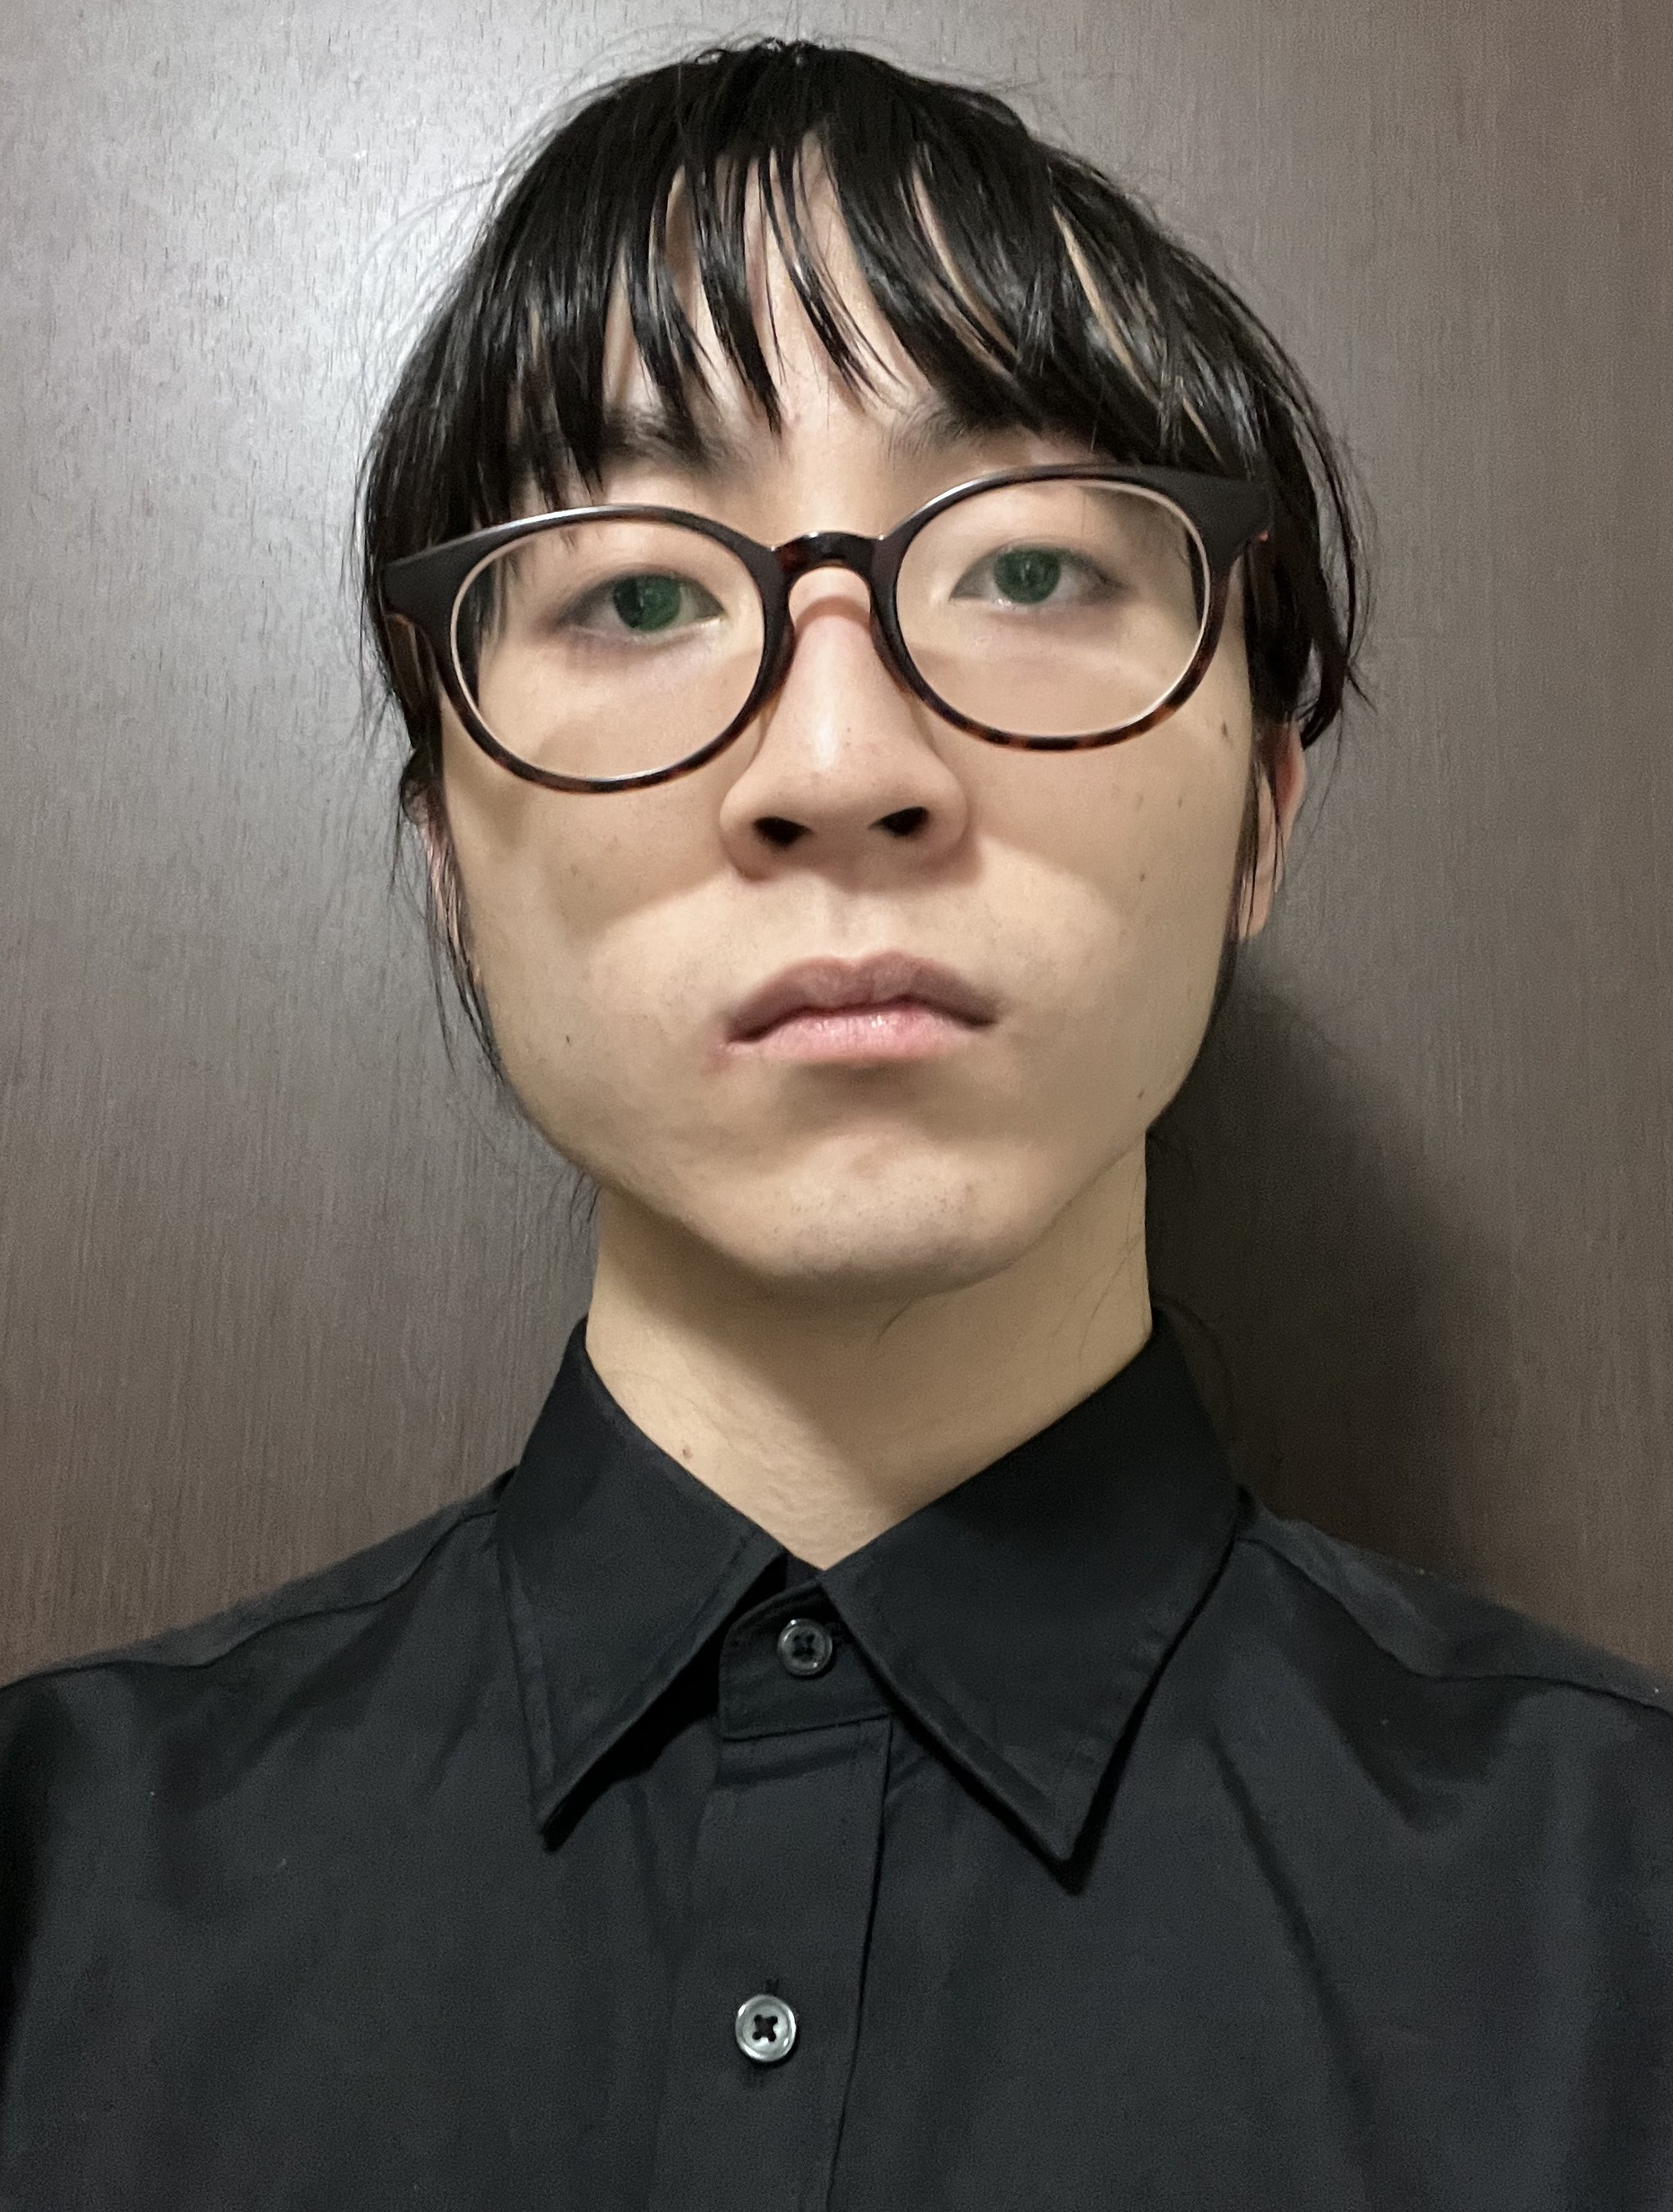
\includegraphics[width=1in,height=1.25in,clip,keepaspectratio]{img/sano2.jpg}}]{Wataru Sano} received the B.E. degree from the Undergraduate School of Computer Science and Engineering, Shibaura Institute of Technology, Tokyo, Japan, in 2024. He is currently pursuing the M.E. degree with the Graduate School of Electric Engineering and Computer Science, Shibaura Institute of Technology. 
\end{IEEEbiography}

\begin{IEEEbiography}[{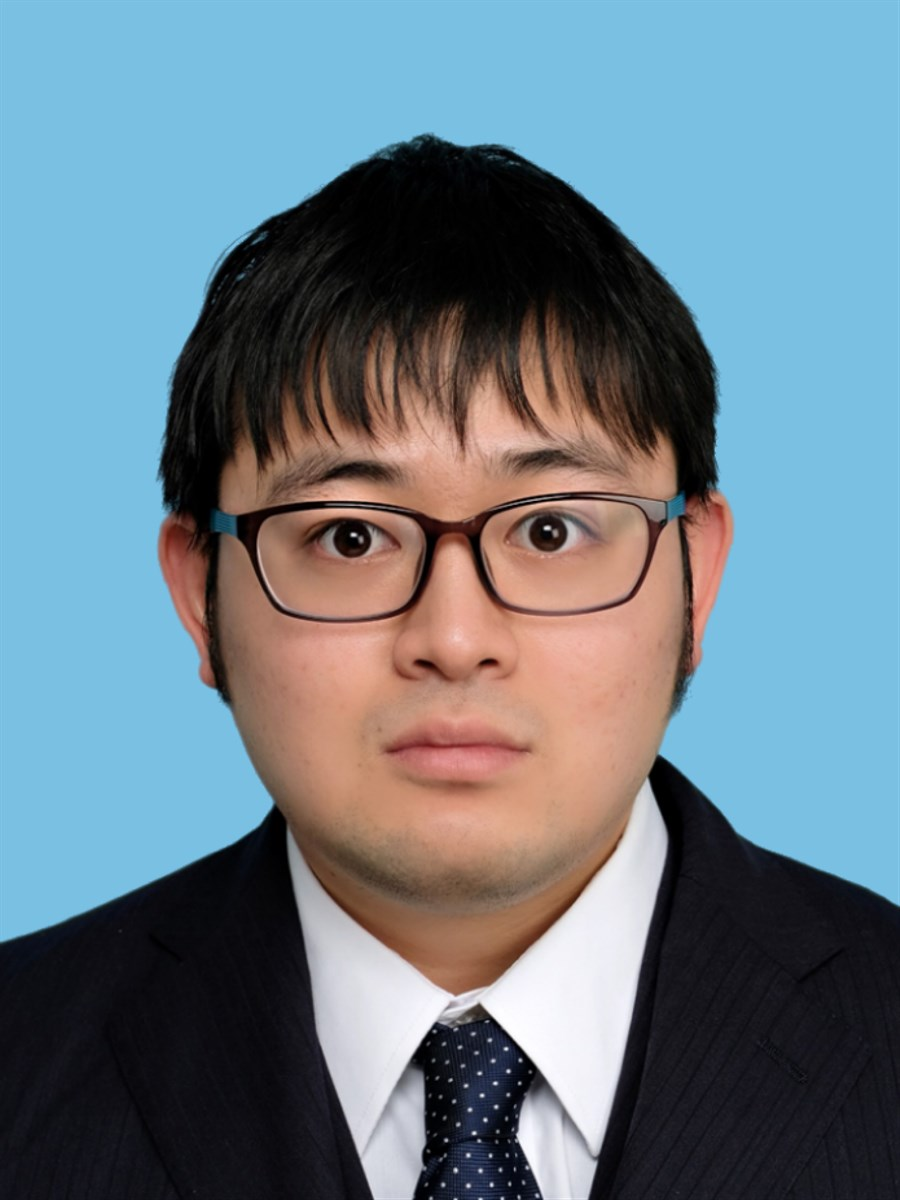
\includegraphics[width=1in,height=1.25in,clip,keepaspectratio]{img/Watanabe.jpg}}]{Jumpei Watanabe} received the B.E. degree from the Undergraduate School of Computer Science and Engineering, Shibaura Institute of Technology, Tokyo, Japan, in 2023.
He received the M.E. degree from the Graduate School of Electrical Engineering and Computer Science, Shibaura Institute of Technology, Tokyo, Japan, in 2025.
\end{IEEEbiography}
  
\begin{IEEEbiography}[{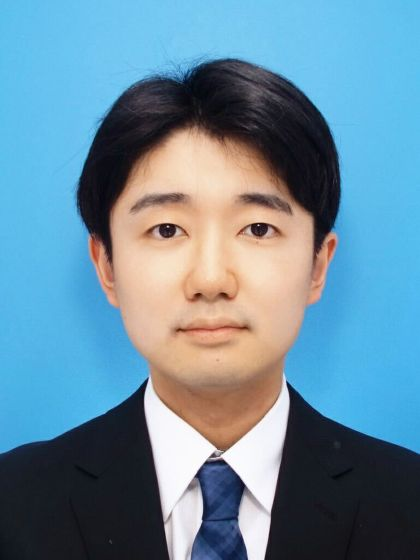
\includegraphics[width=1in,height=1.25in,clip,keepaspectratio]{img/pic_2025.jpg}}]{Haruma Shiraishi}
received the B.E. degree from the
Undergraduate School of Computer Science and Engineering, Shibaura Institute of Technology, Tokyo,
Japan, in 2025. He is currently pursuing the M.E. degree with the Graduate School of Electric Engineering and Computer Science, Shibaura Institute of Technology.
\end{IEEEbiography}

\begin{IEEEbiography}[{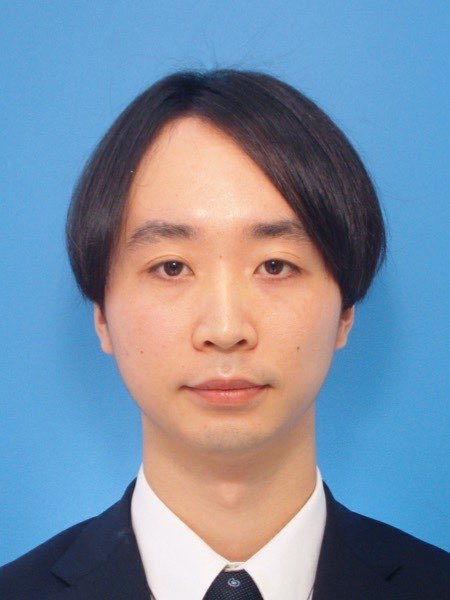
\includegraphics[width=1in,height=1.25in,clip,keepaspectratio]{img/rsugano.jpg}}]{Ryusei Sugano} (Graduate Student Member, IEEE) 
received the M.E. degree with the Graduate School of Electric Engineering and Computer Science, Shibaura Institute of Technology.
He is currently pursuing the Ph.D. degree with the Graduate School of Electric Engineering and Computer Science, Shibaura Institute of Technology.
\end{IEEEbiography}

\begin{IEEEbiography}[{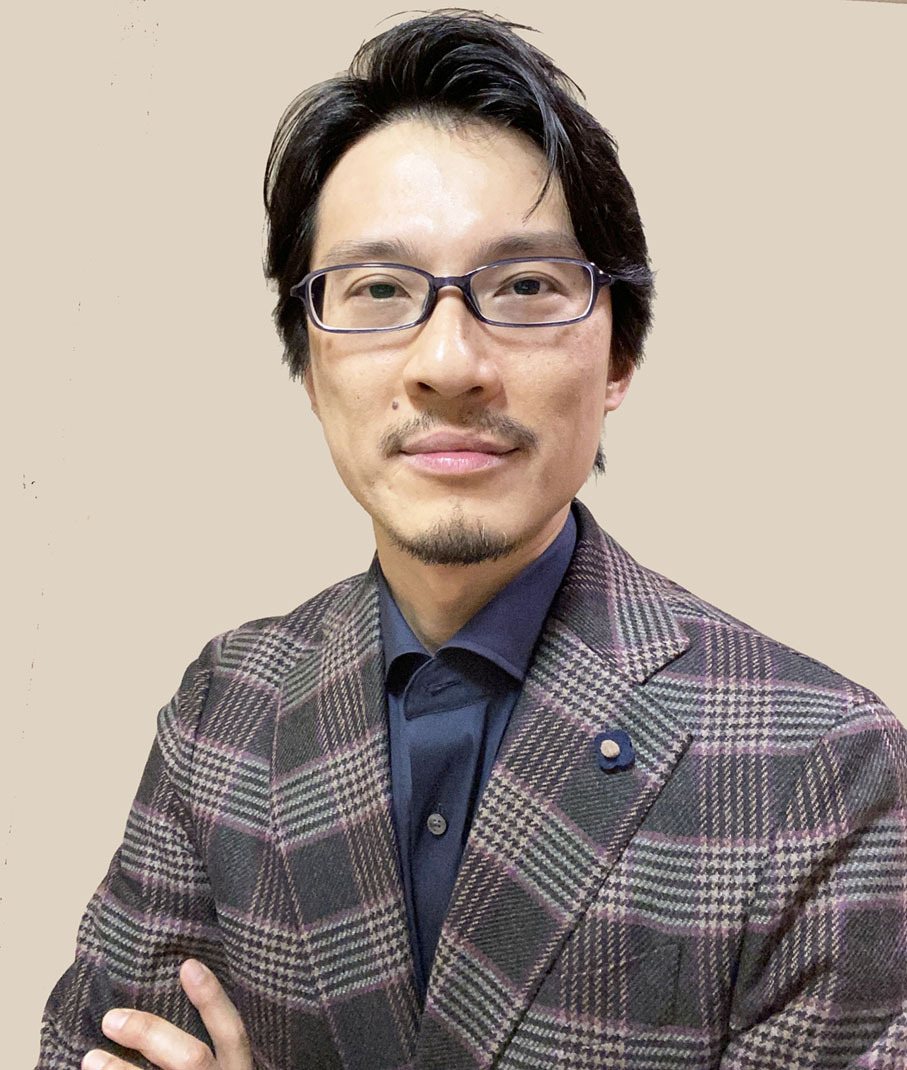
\includegraphics[width=1in,height=1.25in,clip,keepaspectratio]{img/RShinkuma.jpg}}]{Ryoichi Shinkuma} (Senior Member, IEEE) 
received the B.E., M.E., and Ph.D. degrees in communications engineering from Osaka University, Suita, Osaka, Japan, in 2000, 2001, and 2003, respectively. 
He joined the Graduate School of Informatics, Kyoto University, Kyoto, Japan, where he has worked as an Assistant Professor from 2003 to 2011 and an Associate Professor from 2011 to 2021. 
He was a Visiting Scholar with the Wireless Information Network Laboratory, Rutgers University, New Brunswick, NJ, USA, from 2008 to 2009.
In 2021, he joined the Faculty of Engineering, Shibaura Institute of Technology, Tokyo, Japan, as a Professor. 
In May 2022, he founded Hyper Digital Twins (HDT) Company Ltd., Tokyo, where he is currently the CTO. 
\end{IEEEbiography}

\begin{IEEEbiography}[{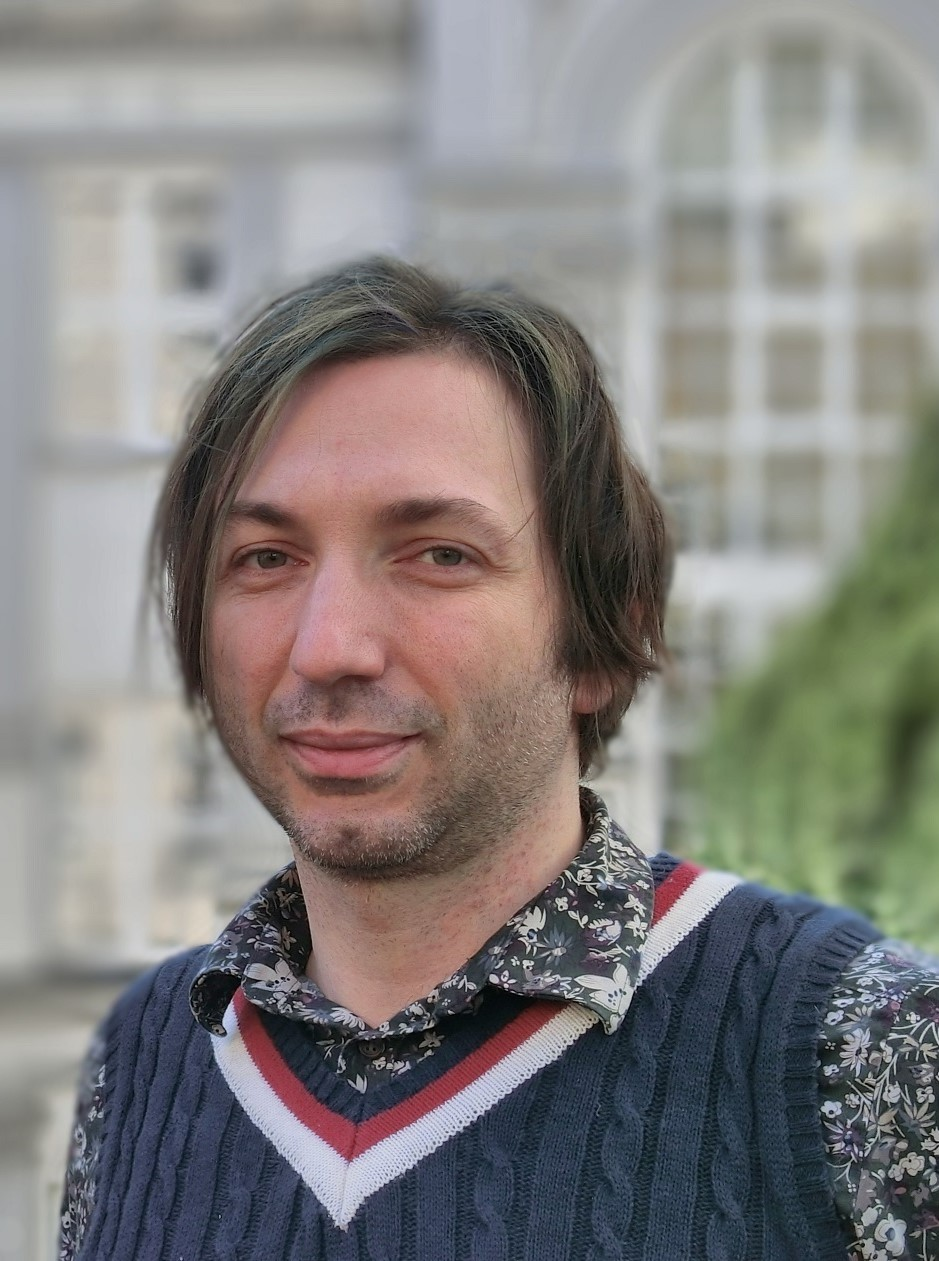
\includegraphics[width=1in,height=1.25in,clip,keepaspectratio]{img/Gab2.jpg}}]{Gabriele Trovato} (Associate Member, IEEE) 
is Associate Professor in Shibaura Institute of Technology, where he is founder and head of LAB 22, and Visiting Researcher in Waseda University, Tokyo, Japan.
He received his M.S. degree in Computer Engineering from the University of Pisa, Italy, and Ph.D. degree in Biorobotics in Waseda University. 
Within the relations between the two countries, Gabriele Trovato has been in the organising committee of Italy-Japan Workshops since 2011, and has been appointed ``Ambassador of Livorno in the world'' by the Municipality of Livorno, Italy.
He has been Visiting Researcher in Karlsruhe Institute of Technology (Germany), University of Sao Paulo (Brazil), PUCP (Peru) and Imperial College London (UK) among others.
\end{IEEEbiography}

\EOD

\end{document}
